\documentclass[twocolumn]{book}
\usepackage[top=1in,bottom=0.5in,left=0.5in,right=0.5in,paperwidth=8.5in,paperheight=11in]{geometry}

%% Math font options
% \usepackage[math]{iwona}
% \usepackage[math]{kurier}
% \usepackage{cmbright}
% \usepackage{lmodern}

%% Font-y stuff



\usepackage{siunitx}
\usepackage{dingbat}
\usepackage[T1]{fontenc}
\usepackage[utf8]{inputenc}
\usepackage{amsfonts}
\usepackage{textcomp}
\usepackage{newtxmath} % Better math lettering (v vs u)
% \usepackage{hyperref} % doesn't work with other packages here


\usepackage{amsmath}

\usepackage{needspace}
%\usepackage{pgfplots}
\usepackage{mdframed}
\usepackage{placeins} % Give float barriers

\usepackage{makeidx}
\usepackage[titles]{tocloft}
\setlength{\cftbeforechapskip}{-0.5ex}

\usepackage{array} % custom column cells
\newcolumntype{M}[1]{>{\centering\arraybackslash}m{#1}}
\setlength{\tabcolsep}{1em}
\renewcommand{\arraystretch}{1.6}



% Better Hyphenation
\usepackage[none]{hyphenat}
\usepackage[english]{babel} % Prevents underscore from causing problems with tex4ht 
% Graphics
\usepackage{graphicx}
\usepackage{xcolor}
\usepackage{maxiplot} % Maxima interface

% Code listings
\usepackage{listings}
\lstset{ %
basicstyle=\ttfamily,
breakatwhitespace=true,
breaklines=true,
tabsize=3
}

\newenvironment{typing}[1]{\begin{figure}[H] \caption{#1} \begin{mdframed}}{\end{mdframed} \end{figure}}
\newenvironment{typingwithlabel}[2]{\begin{figure} \caption{#1} \label{#2} \begin{mdframed}}{\end{mdframed} \end{figure}}

\makeatletter
\@ifpackageloaded{tex4ht}{
\newcommand{\forebook}[1]{#1}
\newcommand{\forprintbook}[1]{}
}{
\newcommand{\forebook}[1]{}
\newcommand{\forprintbook}[1]{#1}
}
\makeatother


\setcounter{tocdepth}{0} % TOC to section level
\setlength{\parindent}{0in} % No paragraph indents
\setlength{\parskip}{10pt} % Between-paragraph skips


\forprintbook{
\def\bookpart#1{%
  \par\newpage\cleardoublepage % Page break
  \thispagestyle{empty}
  \chaptermark{~}
  \sectionmark{~}
  \markboth{~}{~}
  \vspace*{1in} % Vertical shift
  \refstepcounter{part}% Next part
  {\centering\textbf{\Huge Part \thepart}\par}% 
  \addcontentsline{toc}{part}{{\thepart}~~~~~#1}
  \vspace{1cm}% Vertical shift
  {\centering \textbf{\Huge #1}\par}%
  \vspace{2cm}% Vertical shift
  % Some text
}
}

\forebook{
\def\bookpart#1{%
%\section*{~}
%\refstepcounter{part}% Next part
%{\centering\textbf{\Huge Part \thepart}\par}% 
% \part{#1}
% \addcontentsline{toc}{part}{{\thepart}~~~~~#1}
}
}

\forprintbook{
\newenvironment{partintro}{\begin{mdframed}[backgroundcolor=gray!10,skipabove=\baselineskip,skipbelow=\baselineskip]%
~\\ 
}{%
~\\
\end{mdframed}
}
}

\forebook{
\newenvironment{partintro}{}{}
}


% \pgfplotsset{compat=1.10}
\newcommand{\thev}{Th\'{e}venin\ } % Thevenin
\newcommand{\booktitle}[1]{\emph{#1}}
\newcommand{\myamp}{\,\si{\ampere}}
\newcommand{\mymamp}{\,\si{\milli\ampere}}
\newcommand{\myuamp}{\,\si{\micro\ampere}}
\newcommand{\myvolt}{\,\si{\volt}}
\newcommand{\myohm}{\,\si{\ohm}}
\newcommand{\mykohm}{\,\si{\kilo\ohm}}
\newcommand{\myMohm}{\,\si{\mega\ohm}}
\newcommand{\mywatt}{\,\si{\watt}}
\newcommand{\mymwatt}{\,\si{\milli\watt}}
\newcommand{\myuf}{\,\si{\micro\farad}}
\newcommand{\mynf}{\,\si{\nano\farad}}
\newcommand{\mypf}{\,\si{\pico\farad}}
\newcommand{\myf}{\,\si{\farad}}
\newcommand{\myhz}{\,\si{\hertz}}
\newcommand{\mykhz}{\,\si{\kilo\hertz}}
\newcommand{\myhy}{\,\si{\henry}}
\newcommand{\mymhy}{\,\si{\milli\henry}}
\newcommand{\myuhy}{\,\si{\micro\henry}}
\newcommand{\mywb}{\,\si{\weber}}
\newcommand{\myuwb}{\,\si{\micro\weber}}
\newcommand{\mysec}{\textrm{ seconds}}
\newcommand{\deriv}[1]{\mathrm{d}#1}
\newcommand{\pd}[2]{\partial{#1}_{#2}}
\newcommand{\myint}{\int\!}
\renewcommand{\dh}{\deriv{h}}
\newcommand{\dx}{\deriv{x}}
\newcommand{\dy}{\deriv{y}}
\newcommand{\ds}{\deriv{s}}
\newcommand{\dr}{\deriv{r}}
\newcommand{\dt}{\deriv{t}}
\newcommand{\du}{\deriv{u}}
\newcommand{\dv}{\deriv{v}}
\newcommand{\dw}{\deriv{w}}
\newcommand{\diff}{\mathrm{d}}
\newcommand{\dz}{\deriv{z}}
\newcommand{\dq}{\deriv{q}}
\newcommand{\dQ}{\deriv{Q}}
\newcommand{\dV}{\deriv{V}}
\newcommand{\dydx}{\frac{\dy}{\dx}}
\newcommand{\arccot}{\mathrm{arccot}}
\newcommand{\arcsec}{\mathrm{arcsec}}
\newcommand{\arccsc}{\mathrm{arccsc}}
\newcommand{\glossterm}[1]{\textbf{#1}}
\newcommand{\fixme}[1]{FIXME---\textbf{#1}}
\newcommand{\degrees}{^{\circ}}
\renewcommand{\times}{*}

\newcommand{\icode}[1]{\texttt{#1}}


\newcommand\simplepdffigure[3]{
\begin{figure}
\caption{#1}
\label{fig#2}
\centering
\includegraphics[scale=#3]{#2.pdf}
\end{figure}
}

\newcommand\simplegraphicsfigure[3]{
\begin{figure}
\caption{#1}
\label{fig#2}
\centering
\includegraphics[scale=#3]{#2.png}
\end{figure}
}

\newcommand\simplegraph[1]{
	\begin{tikzpicture}
		\begin{axis}[
			xlabel=$x$,
			ylabel=$y$,
			axis equal image
		]
			\addplot+[mark=none,smooth]{#1};
		\end{axis}
	\end{tikzpicture}
}

\newcommand\mxpoutopt[1]{gnuplot_out_file,"./generated_plots\jobname#1.png"}
\newcommand\maxgraphout[1]{\begin{center}\mxpIncludegraphics[scale=0.60]{generated_plots/\jobname#1.png}\end{center}}
\newcommand\maxgraphscale[2]{\begin{center}\mxpIncludegraphics[scale=#2]{generated_plots/\jobname#1.png}\end{center}}
\newcommand\maxdraw[3]{
	\begin{maximacmd}
		draw2d(terminal=eps_color, file_name="generated_plots/\jobname#1", xaxis=true, yaxis=true, yaxis_type=solid, xaxis_type=solid, #2);
	\end{maximacmd}
	\begin{center}
		\mxpIncludegraphics[scale=#3]{generated_plots/\jobname#1.eps}
	\end{center}
}

\newcommand\maxgraph[3]{
	\begin{maximacmd}
		plot2d(#2, #3, [gnuplot_preamble,"set zeroaxis;"], [gnuplot_term, png], [\mxpoutopt{#1}])$
	\end{maximacmd}
	\maxgraphout{#1}
}

\begin{maximacmd}
load(draw);
set_draw_defaults(grid=true, fill_color=grey, xaxis_type=solid, yaxis_type=solid, xlabel="x", ylabel="y");
\end{maximacmd}
% xaxis_color, xaxis_type (solid), xaxis_width, yaxis..., font, font_size, line_width

\newcounter{examplecounter}
\def\theexamplecounter{\thechapter.\arabic{examplecounter}}
\newenvironment{exampleprob}{\begin{quote}%
\refstepcounter{examplecounter}%
\textbf{Example \theexamplecounter}%
\quad
}{%
\end{quote}%
}

\newenvironment{advsidebar}[1]{%
	\begin{sidebar}[Advanced: #1]
}{%
	\end{sidebar}
}

\newenvironment{sidebar}[1][]{%
	\Needspace{10\baselineskip}
	\begin{mdframed}[%
		backgroundcolor=gray!10,
		frametitle={--- \hskip 10pt #1},
		frametitleaboveskip=0pt,
		frametitlebelowskip=10pt,
		innertopmargin=20pt,
		innerbottommargin=10pt,
		shadow=false,
		shadowsize=2pt,
		skipabove=\baselineskip,
		skipbelow=\baselineskip,
		linewidth=0.5pt,
		frametitlerule=true,
		frametitlebackgroundcolor=gray!30
	]%
}{%
	\end{mdframed}
}

\newcommand\reviewsection{\newpage\section*{Review}}
\newcommand\exercisesection{\newpage\section*{Exercises}}
\newcommand{\applysection}{\section*{Apply What You Have Learned}}




\usepackage{xr}
\externaldocument{ElectronicsForEveryone}
\newcommand{\question}[1]{\textbf{Question:} #1 ~\newline~\newline}
\newcommand{\solution}[1]{\textbf{Solution:} #1 ~\newline~\newline}
\newcommand{\explanation}[1]{\textbf{Explanation:} #1 ~\newline~\newline}

\raggedbottom

\begin{document}
\sloppy

\frontmatter
\tableofcontents
\mainmatter

\chapter{Introduction}

This chapter had no questions.

\chapter{Before We Begin}

This chapter had no questions.

\chapter{Dealing with Units}

\begin{enumerate}
\item \fixme{Need questions on this}
\end{enumerate}


\chapter{What is Electricity?}


\begin{enumerate}
\item 
\question{If I have 56 milliamps of current flowing, how many amps of current do I have flowing?}
\solution{$0.056\myamp$}
\explanation{A milliamp is $0.001\myamp$, so, to convert, we multiply milliamps by $0.001$.
$$ 0.001 \frac{\myamp}{\mymamp} \times 56 \mymamp = 0.056\myamp $$
}
\item 
\question{If I have 1,450 milliamps of current flowing, how many amps of current do I have flowing?}
\solution{$1.45\myamp$}
\explanation{A milliamp is $0.001\myamp$, so, to convert, we multiply milliamps by $0.001$.
$$ 0.001 \frac{\myamp}{\mymamp} \times 1450\mymamp = 1.45\myamp $$
}
\item 
\question{If I have 12 amps of current flowing, how many milliamps of current do I have flowing?}
\solution{$12,000\mymamp$}
\explanation{There are $1,000$ milliamps in each amp.  So, to convert, we multiplay amps by $1,000$.
$$ 1,000 \frac{\mymamp}{\myamp} \times 12\myamp = 12,000\mymamp $$
}
\item 
\question{If I have 0.013 amps of current flowing, how many milliamps of current do I have flowing?}
\explanation{There are $1,000$ milliamps in each amp.  So, to convert, we multiplay amps by $1,000$.
$$ 1,000 \frac{\mymamp}{\myamp} \times 0.013\myamp = 12\mymamp $$
}
\item 
\question{If I have 125 milliamps of current flowing for one hour, how many coulombs of charge have I used up?}
\solution{$450\text{ coulombs}$}
\explanation{An amp is a flow of 1 coulomb per second.  First we have to convert milliamps to amps:
$$ 0.001\frac{\myamp}{\mymamp} \times 125 \mymamp = 0.125 \myamp $$
Because an amp is 1 coulomb per second, this is equal to $0.125\frac{\text{coulomb}}{\mysec}$.
Since it is flowing for an hour, we have to convert hours into seconds.
$$ 1 \textrm{ hour} \times \frac{60\text{ min}}{\text{hour}} \times \frac{60\text{ seconds}}{\text{minute}} = 3,600 \text{ seconds} $$
So, we have $0.125$ coulombs per second for $3,600$ seconds.  So the total number of coulombs is:
$$3,600 \frac{\text{coulombs}}{\text{second}} \times 0.125 \text{ seconds} = 450\text{ coulombs} $$
}
\item 
\question{What is the difference between AC and DC current?}
\solution{AC stands for ``alternative current.'' In AC current moves back and forth, continually changing the direction that it is moving.  DC stands for ``direct current.''  In DC current moves in essentially one direction.}
\item 
\question{In AC mains current, how often does the direction of current go back and forth?}
\solution{The direction of current goes back and forth $50--60$ times per second.}
\item 
\question{Why is AC used instead of DC to deliver electricity within a city?}
\solution{There is much less loss over large distances using AC}
\item 
\question{In working with electronic devices, do we normally work in amps or milliamps?}
\solution{With small electronic devices, we usually measure our currents in milliamps.}
\end{enumerate}


\chapter{Voltage and Resistance}


\begin{enumerate}
\item 
\question{If I have a 4-volt battery, how many volts are between the positive and negative terminals of this battery?}
\solution{$4\myvolt$}
\explanation{The definition of a battery's voltage is the number of volts between the positive and negative terminals.}
\item 
\question{If I choose the \emph{negative} terminal of this battery as my ground, how many volts are at the \emph{negative} terminal?}
\solution{$0\myvolt$}
\explanation{Because volts are relative units, a point must be chosen as the ``zero-volt'' level.  This is known as the ground.  Therefore, if the negative terminal is the ground, it is, by definition, zero volts.}
\item 
\question{If I choose the \emph{negative} terminal of this battery as my ground, how many volts are at the \emph{positive} terminal?}
\solution{$4\myvolt$}
\explanation{On a $4\myvolt$ battery, the positive terminal is by definition 4 volts above the negative terminal.  If the negative terminal is the ground (i.e., the zero point), then 4 volts above that will be $4\myvolt$.}
\item 
\question{If I choose the \emph{positive} terminal of this battery as my ground, how many volts are at the \emph{negative} terminal?}
\solution{$-4\myvolt$}
\explanation{On a $4\myvolt$ battery, the positive terminal is by definition 4 volts above the negative terminal. If the positive terminal is the ground (i.e., the zero point), then that is 4 volts above the negative terminal.  That must mean that the negative terminal is 4 volts below zero, or $-4\myvolt$.}
\item 
\question{Given a constant voltage, what effect does increasing the resistance have on current?}
\solution{The current will decrease.}
\explanation{Because $V = I \times R$, with constant voltage increasing the resistance will reduce the current.}
\item 
\question{Given a constant current, what effect does increasing the resistance have on voltage?}
\solution{The voltage will increase.}
\explanation{Because $V = I \times R$, if the current is kept constant, increasing the resistance will increase the voltage.}
\item 
\question{If I have a $10\myvolt$ battery, how much resistance would I need to have a current flow of 10 amps?}
\solution{$1\myohm$}
\explanation{Because we are looking for resistance, we can use Equation~\ref{ohomequationr}.
\begin{align*}
R &= V / I \\
  &= 10 / 10 \\
  &= 1
\end{align*}
We would need a $1\myohm$ resistance.
}
\item 
\question{If I have a 3-volt battery, how much resistance would I need to have a current flow of 15 amps?}
\solution{$0.2\myohm$}
\explanation{We can use Equation~\ref{ohmequationr} to find how much resistance we need:
\begin{align*}
R &= V / I \\
  &= 3 / 15 \\
  &= 0.2
\end{align*}
We would need a $0.2\myohm$ resistance.
}
\item 
\question{Given 4 amps of current flow across 200 ohms of resistance, how much voltage is there in my circuit?}
\solution{$800\myvolt$}
\explanation{This can be solved using Equation~\ref{ohmequationv}:
\begin{align*}
V &= I \times R \\
  &= 4 \times 200 \\
  &= 800
\end{align*}
This circuit has 800 volts.
}
\item 
\question{If I am wanting to limit current flow to 2 amps, how much resistance would I need to add to a 40-volt source?}
\solution{$20\myohm$}
\explanation{This problem can be solved using Equation~\ref{ohmequationr}:
\begin{align*}
R &= V / I \\
  &= 40 / 2 \\
  &= 20
\end{align*}
You would need to add $20\myohm$ of resistance to that source to limit the current flow.
}
\item 
\question{If I am wanting to limit current flow to 2 milliamps, how much resistance would I need to add to a 9-volt source?}
\solution{$4,500\myohm$}
\explanation{Since Ohm's law only works for amps, we need to first convert milliamps to amps:
$$ 0.001 \frac{\myamp}{\mymamp} \times 2 \mymamp = 0.002 \myamp $$
Now we can use Equation~\ref{ohmequationr} to find the resistance we need:
\begin{align*}
R &= V / I \\
  &= 9 / 0.002 \\
  &= 4500
\end{align*}
We would need to add 4500 ohms of resistance to this source to limit the current flow.
}
\item
\question{If I am wanting to limit current flow to 20 milliamps, how much resistance would I need to add to a 5-volt source?}
\solution{$250\myohm$}
\explanation{Since Ohm's law only works for amps, we need to first convert milliamps to amps:
$$ 0.001 \frac{\myamp}{\mymamp} \times 20 \mymamp = 0.02 \myamp $$
Now we can use Equation~\ref{ohmequationr} to find the resistance we need:
\begin{align*}
R &= V / I \\
  &= 5 / 0.02 \\
  &= 250
\end{align*}
We need to add 250 ohms of resistance to this voltage source to limit the current.
}
\end{enumerate}


\chapter{Your First Circuit}


\textbf{Special Note} - In the problems below, since we have not yet studied LED operation in-depth, we are ignoring the electrical characteristics of the LED and just focusing on the resistor.  
If you know how to calculate the circuit characteristics using the LED, please ignore it anyway for the purpose of these exercises.

\begin{enumerate}
\item Calculate the amount of current running in the circuit you built in this chapter using Ohm's law.  Since Ohm's law gives the results in amps, convert the value to milliamps.
\item Let's say that the minimum amount of current needed for the LED to be visibly on is 1 milliamp.  What value of resistor would produce this current?
\item Let's say that the maximum amount of current the LED can handle is 30 milliamps.  What value of resistor would produce this current?
\item Draw a circuit diagram of a short circuit.
\item Take the circuit drawing in this chapter, and modify it so that it is an open circuit.
\item Draw a circuit with just a battery and a resistor.  Make up values for both the battery and the resistor and calculate the amount of current flowing through.
\end{enumerate}


\chapter{Constructing and Testing Circuits}

Note that measured values on a circuit will vary quite a bit because of both the quality of the components and the quality of the multimeter.
For measured results, your values should probably be within 20\% of the values shown here.


All measured values should be measured using the ranging technique discussed in this chapter.

\begin{enumerate}
\item 
\question{Start with the circuit you built in Figure~\ref{figBreadboardBeginFour}.  Measure the voltage drop across the resistor, then measure the voltage drop across the LED.  Now, measure the voltage drop across both of them (put the red multimeter lead on the left side of the resistor and the black multimeter lead on the right side of the LED).  Write down your values.}
\solution{The voltage drop across the LED should be around $1.8\myvolt$.  The voltage drop across the resistor should be around $7.2\myvolt$, but will vary with the battery's current voltage (i.e., how new or old it is).  However, the voltage drop across both of them should be exactly the two of them added together (around $9\myvolt$).}
\item 
\question{Using the same circuit, change the LED from red to blue.   Measure the values again and write them down.  Measure the current going through the circuit using any wire.  Is it the same or different than before?}
\solution{With a blue LED, the voltage drop across the LED should be around $3.3\myvolt$.  The voltage drop across the resistor should be around $5.7\myvolt$, and the voltage drop across both of them should be your two results added together.  The current should be at $5.7\mymamp$.  This should be the case no matter where you test the current.}
\item 
\question{Add another LED in series with the one you have already.  Measure the voltage drops between each side of each component in the circuit.  Measure the current going through any given wire.  Write down each value.}
\solution{This will vary with the color of the LED.  However, in general, it should drop the voltage another $1.8--3.3$ volts.  It will also reduce the current flowing through the circuit.  However, all wires should have the same current going through them.}
\item 
\question{Take the new circuit you built in the previous problem and draw the schematic for the circuit.}
\solution{This may vary a little, but should look something like this:
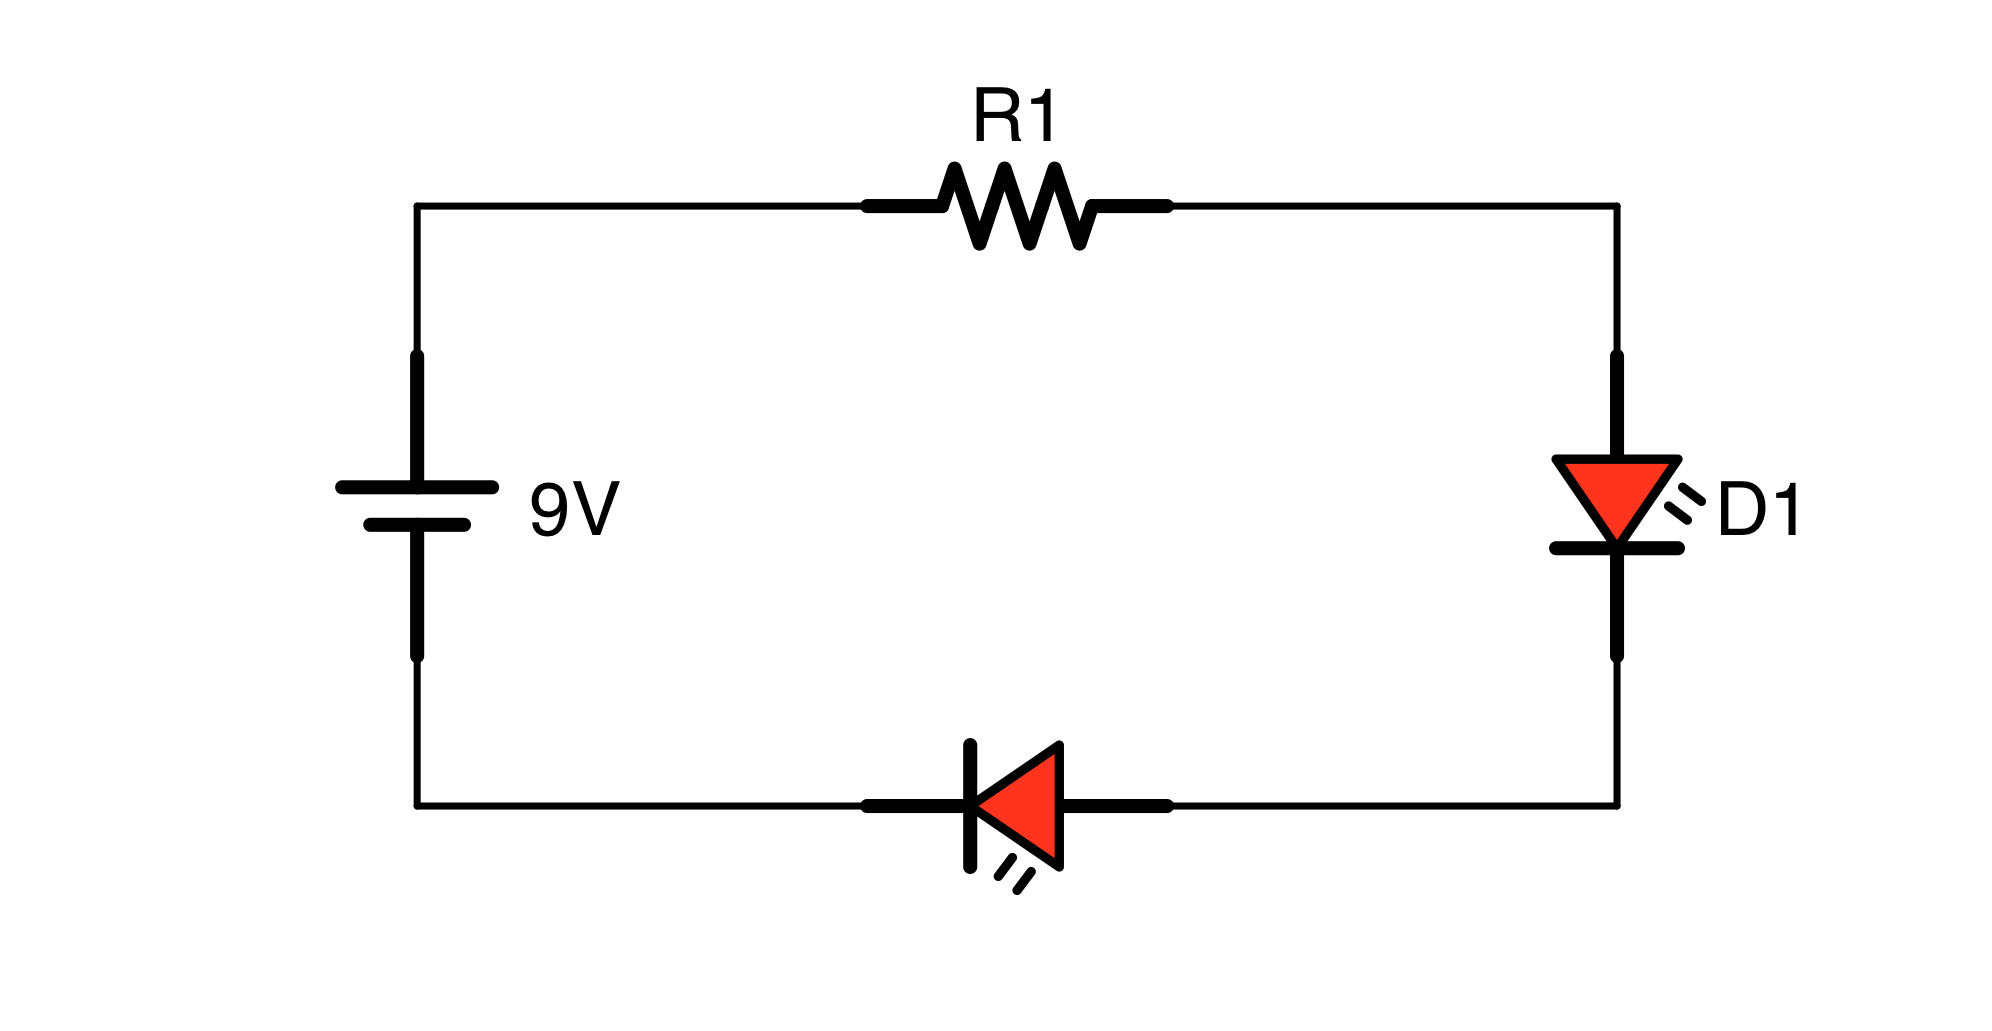
\includegraphics[width=\columnwidth]{SolutionTwoLED.png}
}
\end{enumerate}


\chapter{Analyzing Series and Parallel Circuits}


\begin{enumerate}
\item 
\question{There is a junction in a circuit that has one wire with current flowing in and two wires with current flowing out.  There is $1.25\myamp$ of current coming in, and the first wire going out has $0.15\myamp$ of current going out.  How much current is leaving through the second wire?}
\solution{$1.1\myamp$}
\explanation{The total amount of current leaving must equal the total amount coming in.  If we think of the unknown wire as $x$, we can say that $1.25 = x + 0.15$.  Therefore $x = 1.1\myamp$.}
\item 
\question{There is a junction in a circuit that has two wires with current flowing in and two wires with current flowing out.  The first wire with current flowing in has $0.35\myamp$ of current, the first wire with current flowing out has $0.25\myamp$ of current, and the second wire with current flowing out has $0.42\myamp$ of current.  How much current is flowing in on the second incoming wire?}
\solution{$0.32\myamp$}
\explanation{The total amount of current coming in must equal the total amount leaving.  We have two wires coming in and two wires going out.  The total going out is $0.25 + 0.42 = 0.67\myamp$.
The total coming in must equal that.  We know that one wire has $0.35\myamp$ coming in.  
Since the totals coming in must equal the total going out, we can say that $0.35 + x = 0.67$.
Therefore, our unknown wire must be $0.32\myamp$. }
\item 
\question{At a junction of four wires, wire 1 has $0.1\myamp$ of current flowing in, wire 2 has $0.2\myamp$ of current flowing in, and wire 3 has $0.4\myamp$ of current flowing out.  Is the current in wire 4 going in or out?  How much current is flowing on it?}
\solution{The current in wire 4 is going in with $0.1\myamp$ of current.}
\explanation{The total amount of current coming in must equal the total amount leaving.  Wire 1 and 2 have current coming in.  So, we can add them together and find that together they bring $0.1 + 0.2 = 0.3\myamp$ of current coming in.  Wire 4 has $0.4\myamp$ of current flowing out.  Since that is greater than the amount of current coming in, that means the last wire must have current flowing in.  The amount is $0.4 - 0.3 = 0.1\myamp$.  Therefore, wire 4 has $0.1\myamp$ of current going in.}
\item 
\question{If I have three $100\myohm$ resistors in series, what is the total resistance of the series?}
\solution{$300\myohm$}
\explanation{Resistance in series just adds together.  So we have $100 + 100 + 100 = 300\myohm$ resistance.}
\item 
\question{If I have a $10\myohm$ resistor, a $30\myohm$ resistor, and a $65\myohm$ resistor in series, what is the total resistance of the series?}
\solution{$105\myohm$}
\explanation{Resistance in series just adds together.  So we have $10 + 30 + 65 = 105\myohm$ total resistance in this series.}
\item 
\question{If I have a $5\myohm$ resistor and a $7\myohm$ resistor in series, what is the total resistance of the series?}
\solution{$12\myohm$}
\explanation{Resistance in series just adds together.  So we have $5 + 7 = 12\myohm$ resistance in this series.}
\item 
\question{If I have two resistors in parallel, a $30\myohm$ resistor and a $40\myohm$ resistor, what is the total resistance of this circuit?}
\solution{$17.14\myohm$}
\explanation{Equation~\ref{eqparallelresistancen} tells us how to add together parallel resistance:
\begin{align*}
R_T &= \frac{1}{\frac{1}{30} + \frac{1}{40}} \\
    &\approx \frac{1}{0.03333 + 0.025} \\
    &\approx \frac{1}{0.05833} \\
    &\approx 17.14 \myohm
\end{align*}
}
\item 
\question{If I have three resistors in parallel---$25\myohm$, $40\myohm$, and $75\myohm$, what is the total resistance of this circuit?}
\solution{$12.77\myohm$}
\explanation{Equation~\ref{eqparallelresistancen} tells us how to add together parallel resistance:
\begin{align*}
R_T &= \frac{1}{\frac{1}{25} + \frac{1}{40} + \frac{1}{75}} \\
    &\approx \frac{1}{0.04 + 0.025 + 0.0133} \\
    &\approx \frac{1}{0.0783}
    &\approx 12.77 \myohm
\end{align*}
}
\item 
\question{If I have four resistors in parallel---$1,000\myohm$, $800\myohm$, $2,000\myohm$, and $5,000\myohm$, what is the total resistance of this circuit?}
\solution{$338.98\myohm$}
\explanation{Equation~\ref{eqparallelresistancen} tells us how to add together parallel resistance:
\begin{align*}
R_t &= \frac{1}{\frac{1}{1,000} + \frac{1}{800} + \frac{1}{2,000} + \frac{1}{5,000}} \\
    &= \frac{1}{0.001 + 0.00125 + 0.0005 + 0.0002} \\
    &= \frac{1}{0.00295} \\
    &\approx 338.98\myohm
\end{align*}
}
\item 
\question{If I have three resistors in parallel---$100\myohm$, $5,000\myohm$, and $10,000\myohm$---what is the total resistance of this circuit?  Which of the resistors is the total resistance most similar to?}
\solution{$97.09\myohm$---this is very similar to the $100\myohm$ resistor.}
\explanation{Equation~\ref{eqparallelresistancen} tells us how to add together parallel resistance:
\begin{align*}
R_T &= \frac{1}{\frac{1}{100} + \frac{1}{5,000} + \frac{1}{10,000}} \\
    &= \frac{1}{0.01 + 0.0002 + 0.0001} \\
    &= \frac{1}{0.0103} \\
    &\approx 97.09\myohm
\end{align*}
This is very close to the $100\myohm$ resistance. 
Parallel resistance is always lower (even if slightly) than the lowest parallel resistance.
}
\item 
\question{Take a look at the following circuit diagram.  If the voltage drop between B and C is 2 volts, and the voltage drop between C and D is 3 volts, what is the voltage drop between A and E?  What is the voltage at E?  What is the voltage at A? \\ 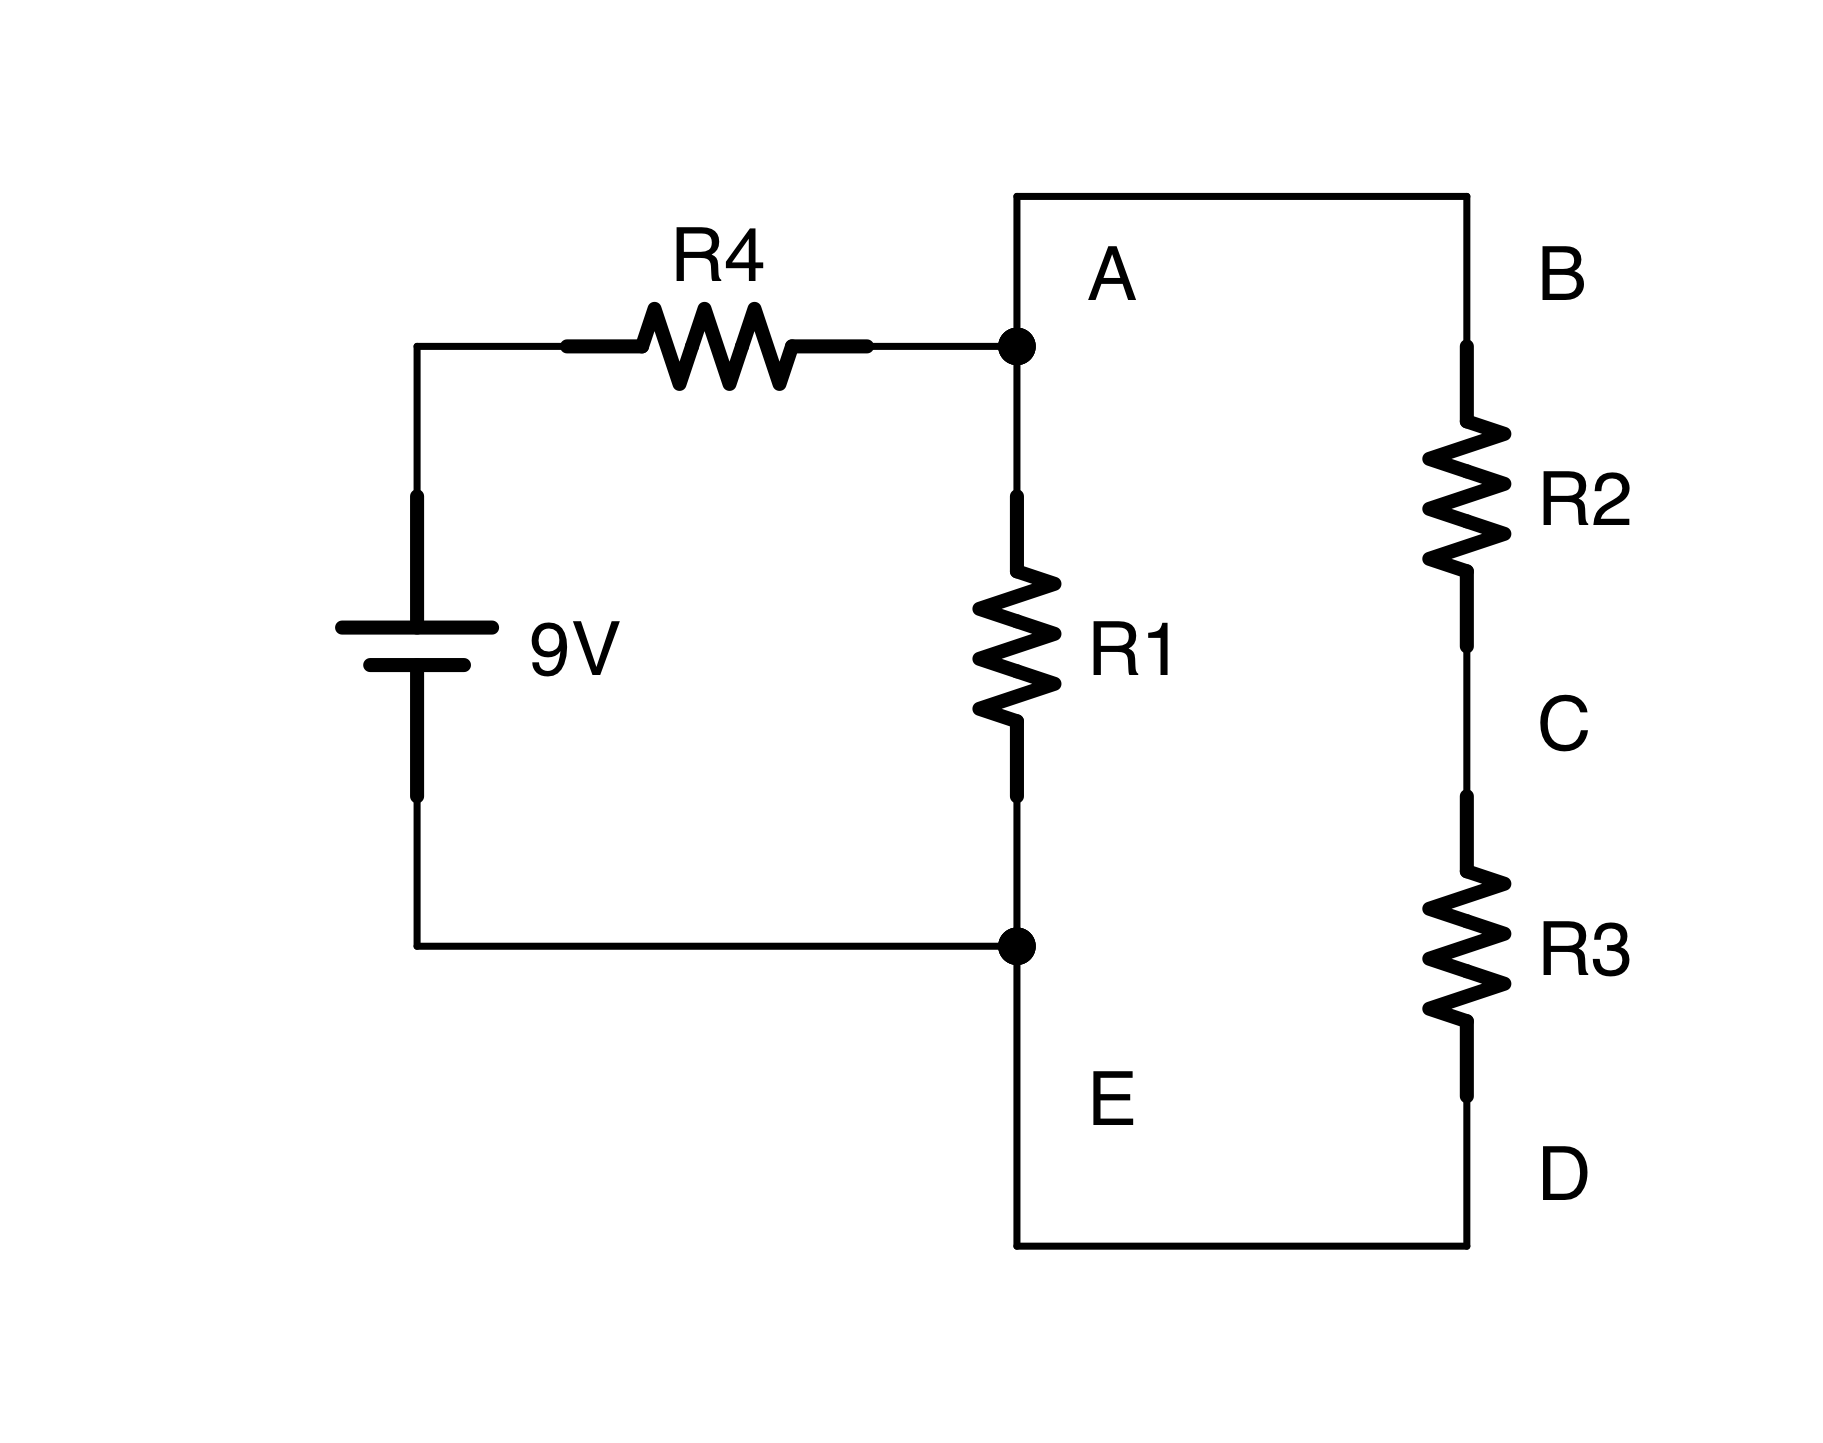
\includegraphics[scale=0.08]{VoltageDropProblem.png}}
\solution{Voltage drop between A and E is $5\myvolt$.  Voltage at E is $0\myvolt$.  Voltage at A is $5\myvolt$.}
\explanation{The voltage starts at $9\myvolt$.  
Every path from the positive of the battery to the ground must take $9\myvolt$.  
Kirchoff's Voltage Law states that every path between every two points must be the same voltage drop.
The path from A to E can take two different routes (either through R1 or through both R2 and R3) but they will \emph{both} have the same voltage drop because of Kirchoff's Voltage Law.
Therefore, since the drop across R2 is $2\myvolt$ and the drop across R3 is $3\myvolt$, the total drop is $2 + 3 = 5\myvolt$.
This is the same no matter what path you travel, so the voltage drop across R1 must also be $5\myvolt$.

So the voltage drop from A to E is $5\myvolt$.

There is no resistor between E and the ground terminal.  That means that these voltages are the same.  Therefore the voltage at E is $0\myvolt$.

Because the voltage at E is zero, the voltage at A is $5\myvolt$ above that, which is $5\myvolt$.
}
\item 
\question{If the circuit above runs with $2\myamp$ total current, what is the value of the resistor R4?}
\solution{$2\myohm$}
\explanation{Since we are imagining $2\myamp$ coming out of the battery (just to note---it is unrealistic for a battery to supply even $1\myamp$), the entire $2\myamp$ will go through resistor R4.

Now, at the end of R4, we determined that the voltage is $5\myvolt$.
Since we started with $9\myvolt$ that means that R4 had to drop us $4\myvolt$.
We can use Ohm's Law to figure out how much resistance was in that resistor:
\begin{align*}
R &= V / I \\
  &= 4 / 2 \\
  &= 2\myohm
\end{align*}
So, R4 is $2\myohm$.
}
\item 
\question{The circuit below is a combination of series and parallel resistances.  Each resistor is labelled with its resistance value, given in ohms.  Find out how much current is flowing through each resistor, and how much each resistor drops the voltage.  \\ 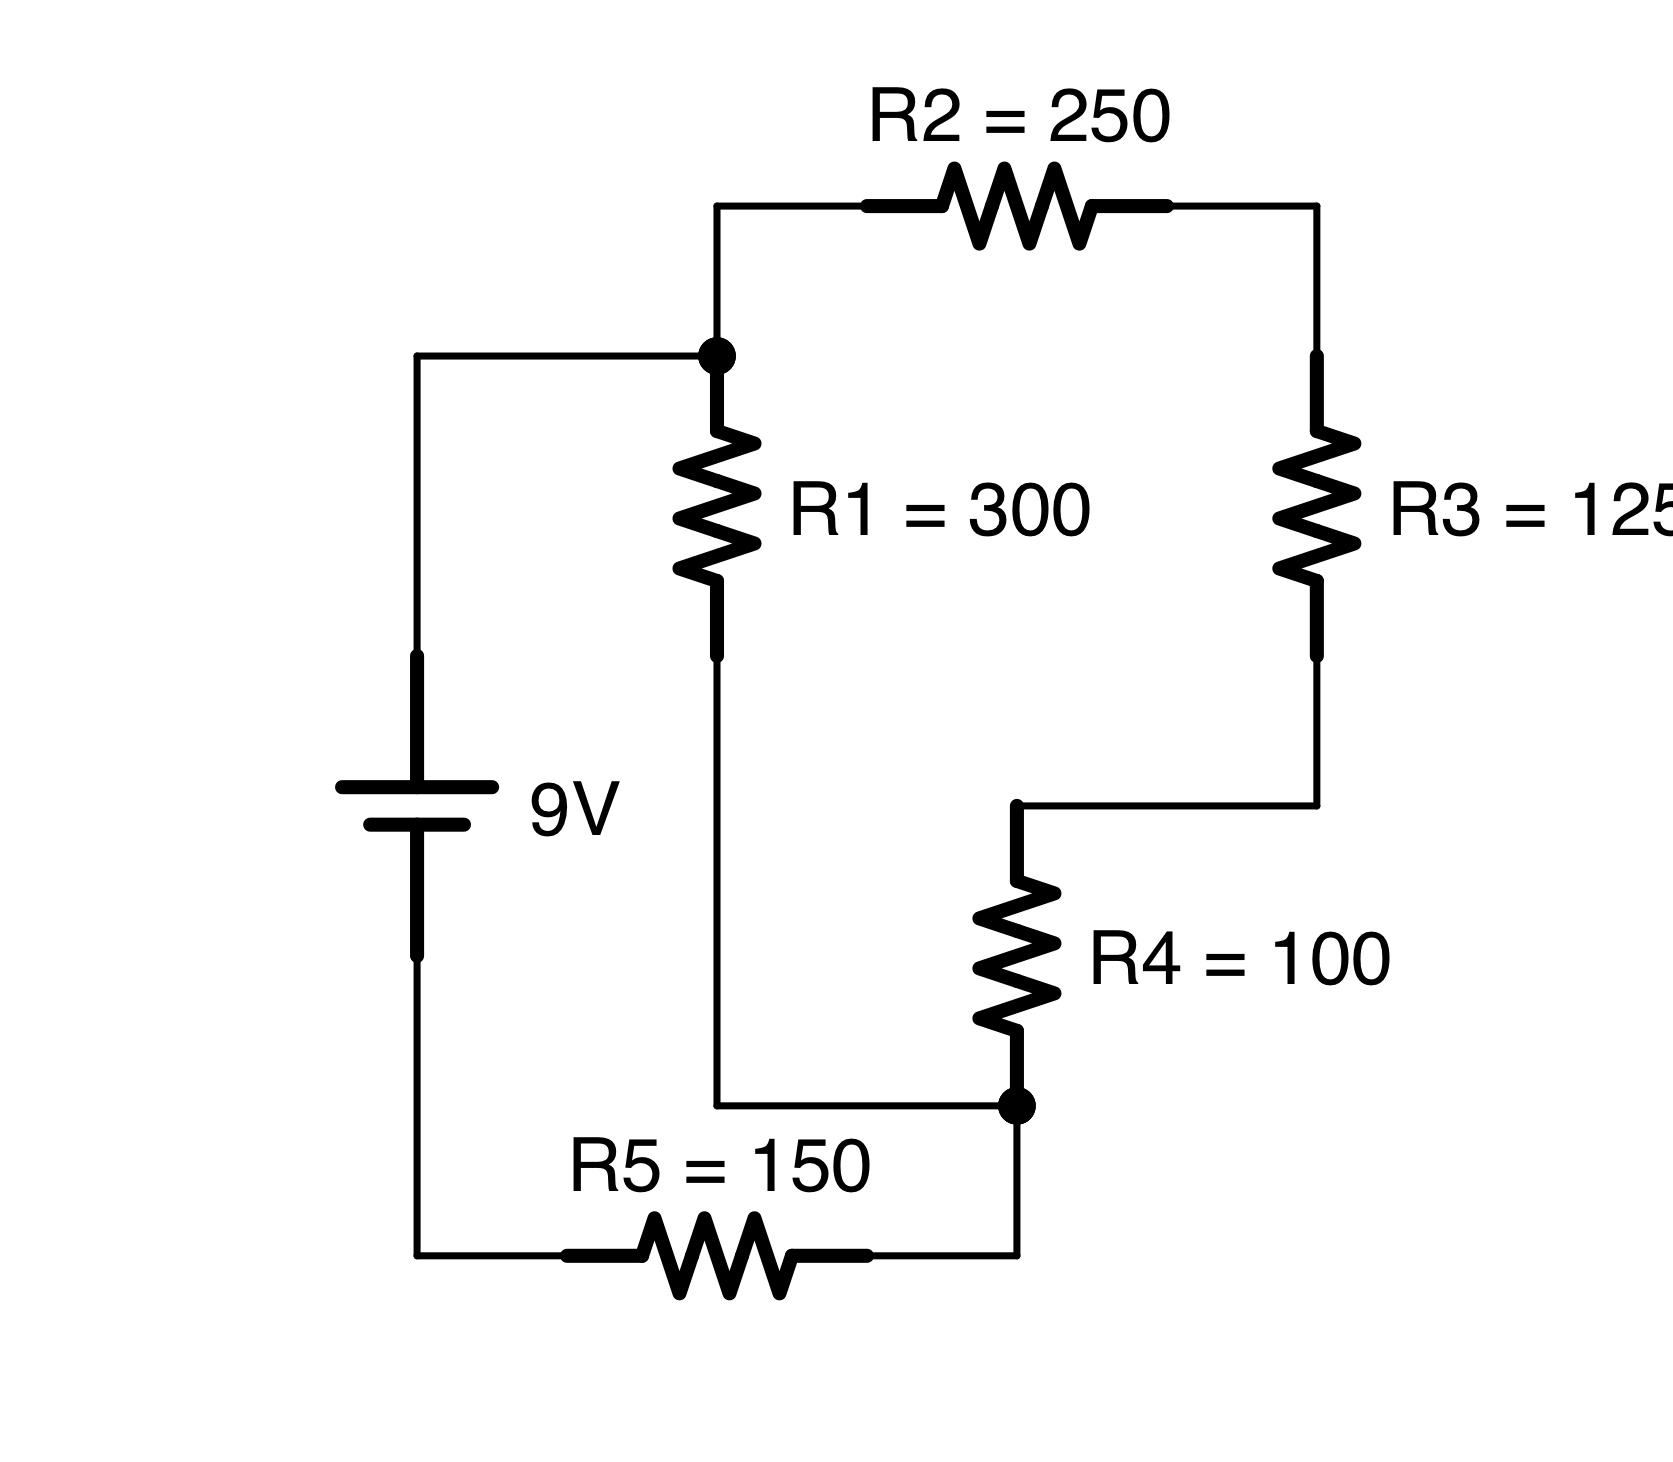
\includegraphics[scale=0.08]{ProblemCalculateCurrentAndVoltage.png}}
\solution{\begin{description}
\item[R1] $4.95\myvolt$ and $0.0165\myamp$
\item[R2] $2.625\myvolt$ and $0.0105\myamp$
\item[R3] $1.3125\myvolt$ and $0.0105\myamp$
\item[R4] $1.05\myvolt$ and $0.0105\myamp$
\item[R5] $4.05\myvolt$ and $0.025\myamp$
\end{description}
Note that these do not exactly add up correctly (because of rounding issues), but that is perfectly normal.  If you are within 1\% of the right answer, you are most likely more accurate than your equipment supports.
}
\explanation{Every circuit like this, no matter how complicated, can be solved by just breaking it down a piece at a time, and solving for each piece as you go.
The most straightforward way to solve these is to first add up \emph{all} of the resistances to get a total resistance, and then solve for total current.  
After that, you can go back through the circuit to find the individual currents and voltages.

So, the easiest way to start adding up the resistors is to take all of the resistors that are in series, and replace them with a single resistance that is the total of them.
Notice that R2, R3, and R4 are all in series with each other with no branches.
Therefore, we can replace these resistors with a single resistor that just adds up the resistances.
So, that segment has a total resistance of $250 + 125 + 100 = 475\myohm$.

That segment is in parallel with R1.
Therefore, we can use the parallel resistance rule to combine these resistances:
\begin{align*}
R_T &= \frac{1}{\frac{1}{300} + \frac{1}{475}} \\
    &\approx \frac{1}{0.00333 + 0.00211} \\
    &\approx \frac{1}{0.00544} \\
    &\approx 183.82\myohm
\end{align*}
Therefore, the whole top network---R1, R2, R3, and R4---can be replaced by a single resistance, $183.82\myohm$.
This network is in series with R5.
Therefore, we can just add these resistances together: $183.82 + 150 = 333.82\myohm$.

That's the whole resistance of the whole circuit.
We know the total voltage drop of the whole circuit, because, by definition, a $9\myvolt$ battery supplies $9\myvolt$ to the circuit.
Therefore, Ohm's Law will give us the total current:
\begin{align*}
I &= V / R \\
  &= 9 / 333.82 \\
  &= 0.0270 \myamp
\end{align*}
The battery will put out $0.027\myamp$ (i.e., $27\mymamp$) of current to this circuit.

Now we need to figure out currents and voltages to each individual component.
R5 is the easiest one to start with because it is directly connected in series with the battery terminal.
That means that all of the current will go through this resistor.
So this resistor is getting $0.027\myamp$.
We can find the voltage drop with Ohm's Law:
$$ V = I * R = 0.027 * 150 = 4.05\myvolt $$

So the current through R5 is $0.027\myamp$ and the voltage drop is $4.05\myvolt$.
That means that the voltage drop through the rest of the network is $4.95\myvolt$.
We can use that to find the currents flowing through here.

The voltage drop across R1 is $4.95\myvolt$ and the resistance is $300\myohm$.  
Therefore, the current is:
$$ I = V / R = 4.95 / 300 = 0.0165\myamp $$
Therefore, R1 has $0.0165\myamp$ flowing through it.
Since we started with $0.027\myamp$, that means the rest of the current must be flowing through the other junction.
So, the right-hand-side of the network has $0.027 - 0.0165 = 0.0105\myamp$ of current flowing through it.
Since R2, R3, and R4 are all in series, that means they all have this same current flowing through them.
To find voltages, we just use Ohm's Law:
\begin{align*}
V_{R2} &= I * R = 0.0105 * 250 = 2.625\myvolt \\
V_{R3} &= I * R = 0.0105 * 125 = 1.3125 \myvolt \\
V_{R4} &= I * R = 0.0105 * 100 = 1.05 \myvolt
\end{align*}
Note that this total voltage is actually slightly higher than what we were looking for (these add up to $4.9875\myvolt$ instead of $4.95\myvolt$ like we were expecting), but being off on the decimal point is normal when we do as much rounding as we have been.
}
\item 
\question{Build the circuit in Figure~\ref{figParallelUsingBreadboard} on your own breadboard.  Measure the voltage drops across every component, and measure the amount of current flowing into the first series resistor.}
\solution{The actual voltage drops will depend on the specific resistor values and colors of your LED.  However, in general you should have between 5 and 40 $\mymamp$ flowing through any part of your circuit.
Additionally, every complete path from positive to ground should be $9\myvolt$ (or whatever size battery you are using).}
\end{enumerate}


\chapter{Diodes and How to Use Them}


\begin{enumerate}
\item If you have a $9\myvolt$ voltage source, a blue LED, and a $500\myohm$ resistor all in series, how much current is running through the LED?
\item If you have a $3\myvolt$ voltage source and a red LED, what size resistor do you need to put in series with the LED to have it use $3\mymamp$ of current?
\item If you have a $10\myvolt$ voltage source, a blue LED, a red LED, and a $200\myohm$ resistor all in series, how much current is running through the LEDs?
\item If I have a $12\myvolt$ voltage source, a blue LED, and a red LED, and the LEDs have a maximum current of $30\mymamp$ before it breaks and a minimum current of $1\mymamp$ before it turns on, what range of resistors can I put in series with the LEDs to get them to light up without breaking?
\item In the circuit below, calculate the how much current flowing through each component and each component's voltage drop if R1 is $500\myohm$. \\ 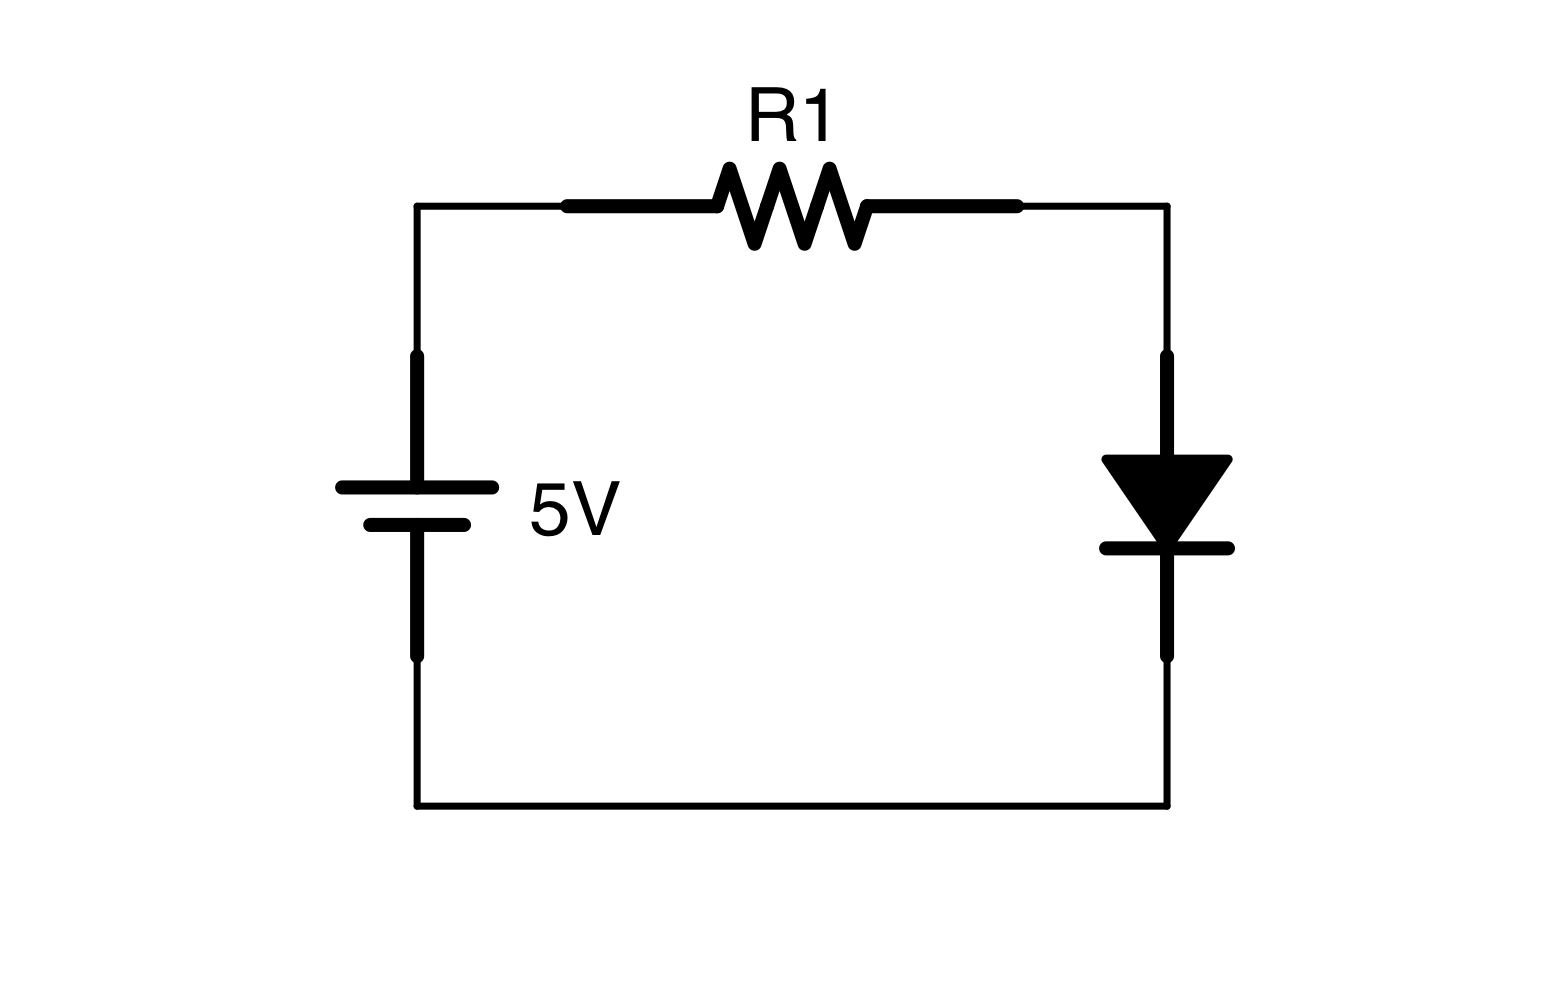
\includegraphics[scale=0.08]{DiodeApplyEx1.png}
\item Let's say instead of a standard diode, the diode is a blue LED.  Recalculate the current going through each component and the voltage drops for each component.
\item In the circuit below, calculate how much current is flowing through each component and each component's voltage drop if R1 is $300\myohm$, R2 is $400\myohm$, and R3 is $500\myohm$.  \\ 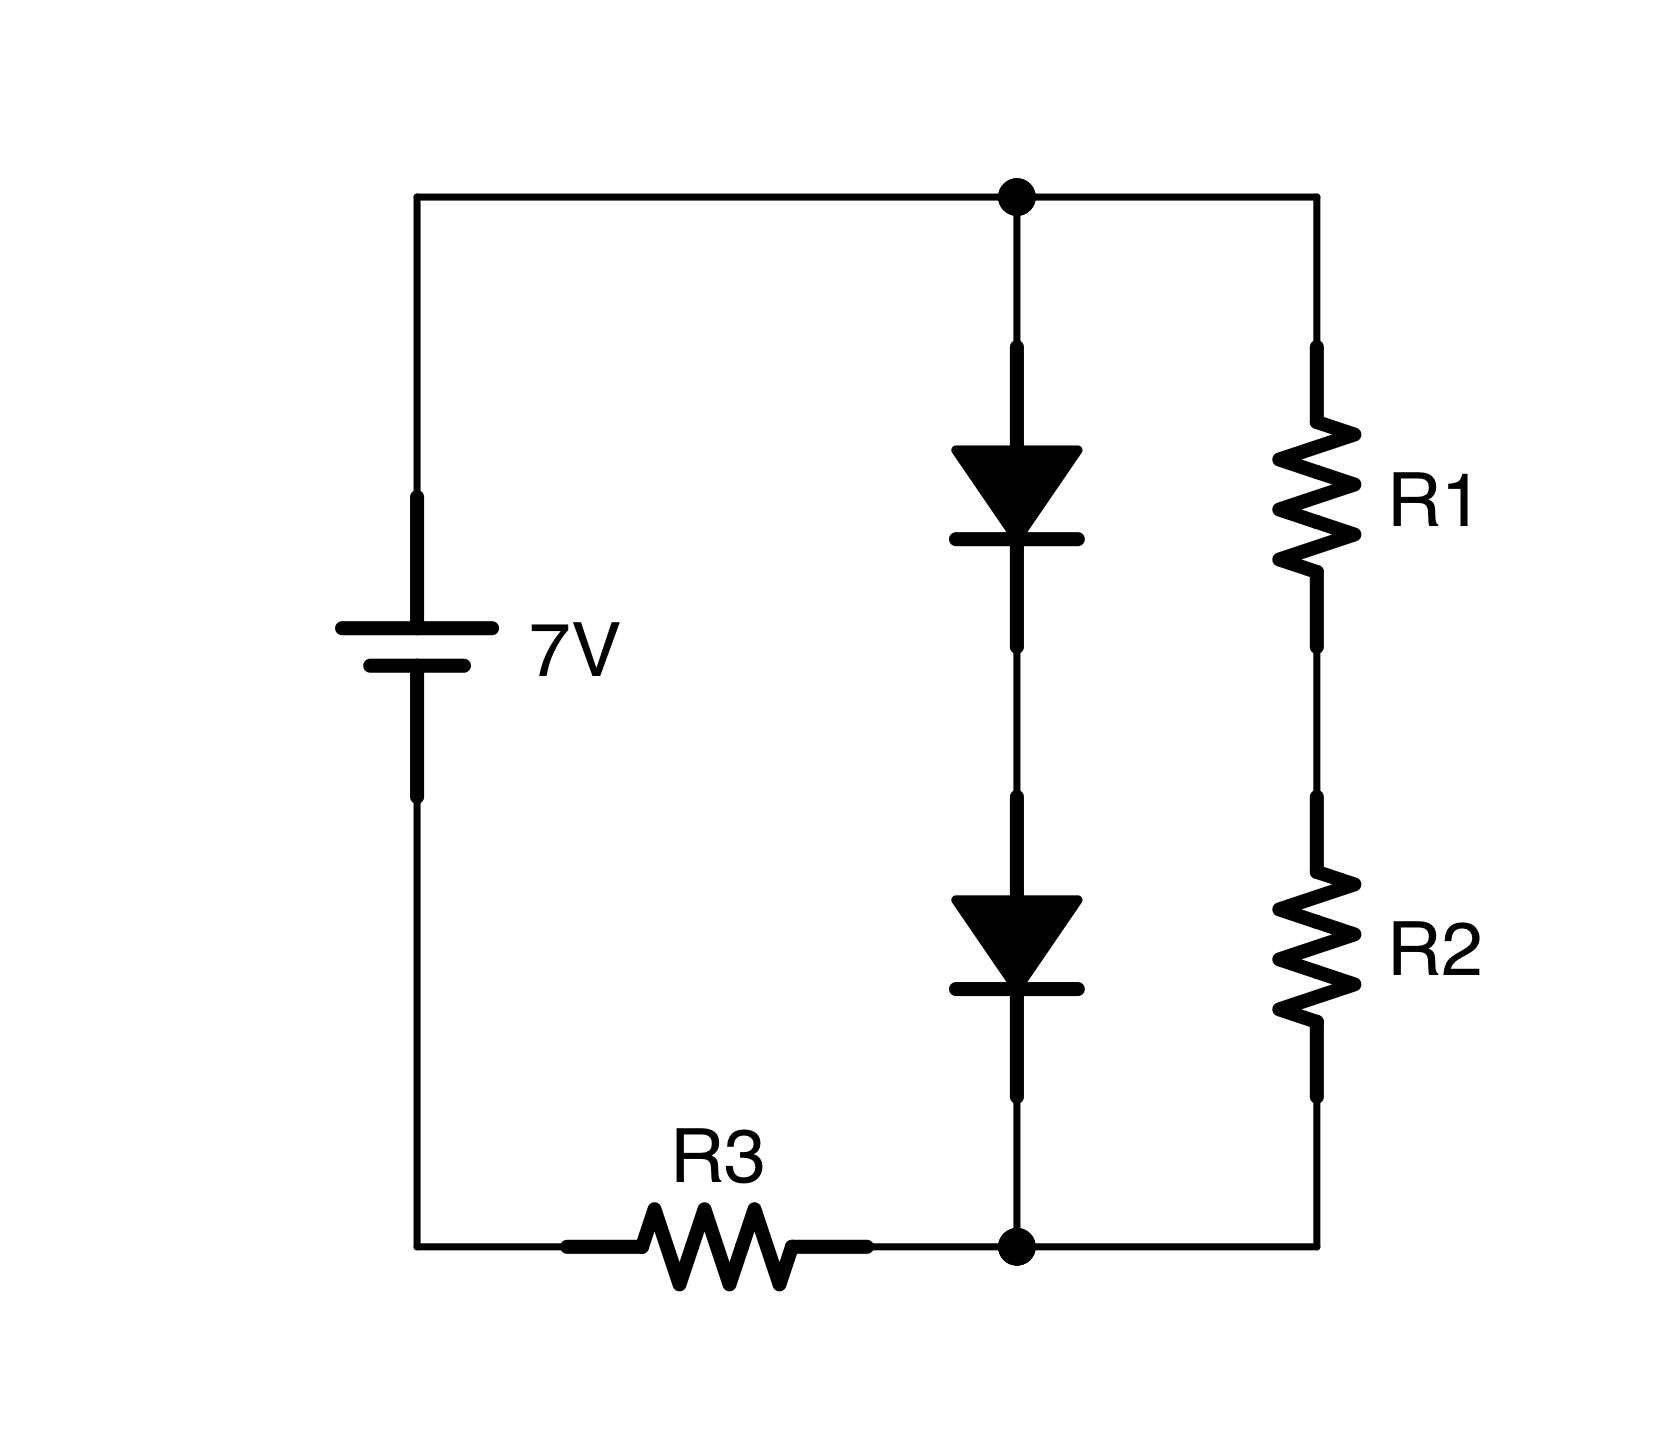
\includegraphics[scale=0.08]{DiodeApplyEx2.png}
\item Draw a circuit that provides a 6-volt regulated power supply to circuit load from a 9-volt battery using regular diodes.  Choose a resistor that works efficiently for a circuit load of $500\myohm$ and operates with a battery voltage from $7\myvolt$ to $9.6\myvolt$.  What is the current at the lowest and highest ranges of the battery?  How much is used by the circuit load and how much is wasted through the diodes in each configuration?
\item Draw an equivalent circuit to the previous question using a Zener diode instead of normal diodes.
\end{enumerate}


\chapter{Basic Resistor Circuit Patterns}


\begin{enumerate}
\item 
\question{In Figure~\ref{figMultipleSwitches}, calculate the amount of current used by the whole circuit for each configuration of the switches S2 and S3 when S1 is closed.  You can assume that the LEDs are red LEDs.}
\solution{\begin{description}
\item[S2 closed] 9\mymamp 
\item[S3 closed] 4.5\mymamp
\item[Both closed] 13.5\mymamp
\end{description}}
\explanation{Because these circuit branches are in parallel, the total current is the sum of the individual currents.  
Because both branches connect to both positive and negative without going through resistance, then they each start at $9\myvolt$ and connect to ground, so they each use a full $9\myvolt$.
Therefore, we can use Ohm's Law to calculate the amount of current going through each branch:
\begin{align*}
I_{S2} &= V / R \\
       &= 9 / 1000 \\
       &= 0.009\myamp = 9\mymamp \\
I_{S3} &= V / R \\
       &= 9 / 2000 \\
       &= 0.0045\myamp = 4.5 \mymamp
\end{align*}
Therefore, when S2 is closed, that branch uses $9\mymamp$ of current, and when S3 is closed that branch uses $4.5\mymamp$ of current.
Since they are in parallel and both connected on both sides to the battery, when they are closed they both use $9 + 4.5 = 13.5\mymamp$ of current.
}
\item 
\question{Build the circuit given in Figure~\ref{figMultipleSwitches} (you may swap out resistors with different but similar values---anything from $300\myohm$ to about $5\mykohm$ should work).}
\solution{Since this is a building exercise, the question is whether or not it works correctly.}
\item 
\question{Given a $15\myvolt$ voltage supply, what size of a resistor would be needed to make sure that a circuit never went over $18\mymamp$.}
\solution{$833.33\myohm$}
\explanation{This can be figured out using Ohm's Law.  We simply figure out the resistance needed for $18\mymamp$ ($0.018\myamp$).
\begin{align*}
R &= V / I \\
  &= 15 / 0.018 \\
  &= 833.33\myohm
\end{align*}
}
\item 
\question{Given a $9\myvolt$ battery source, design a voltage divider that will output $7\myvolt$ to a load that has a resistance of $10\mykohm$.}
\solution{The general voltage divider circuit can be seen here:
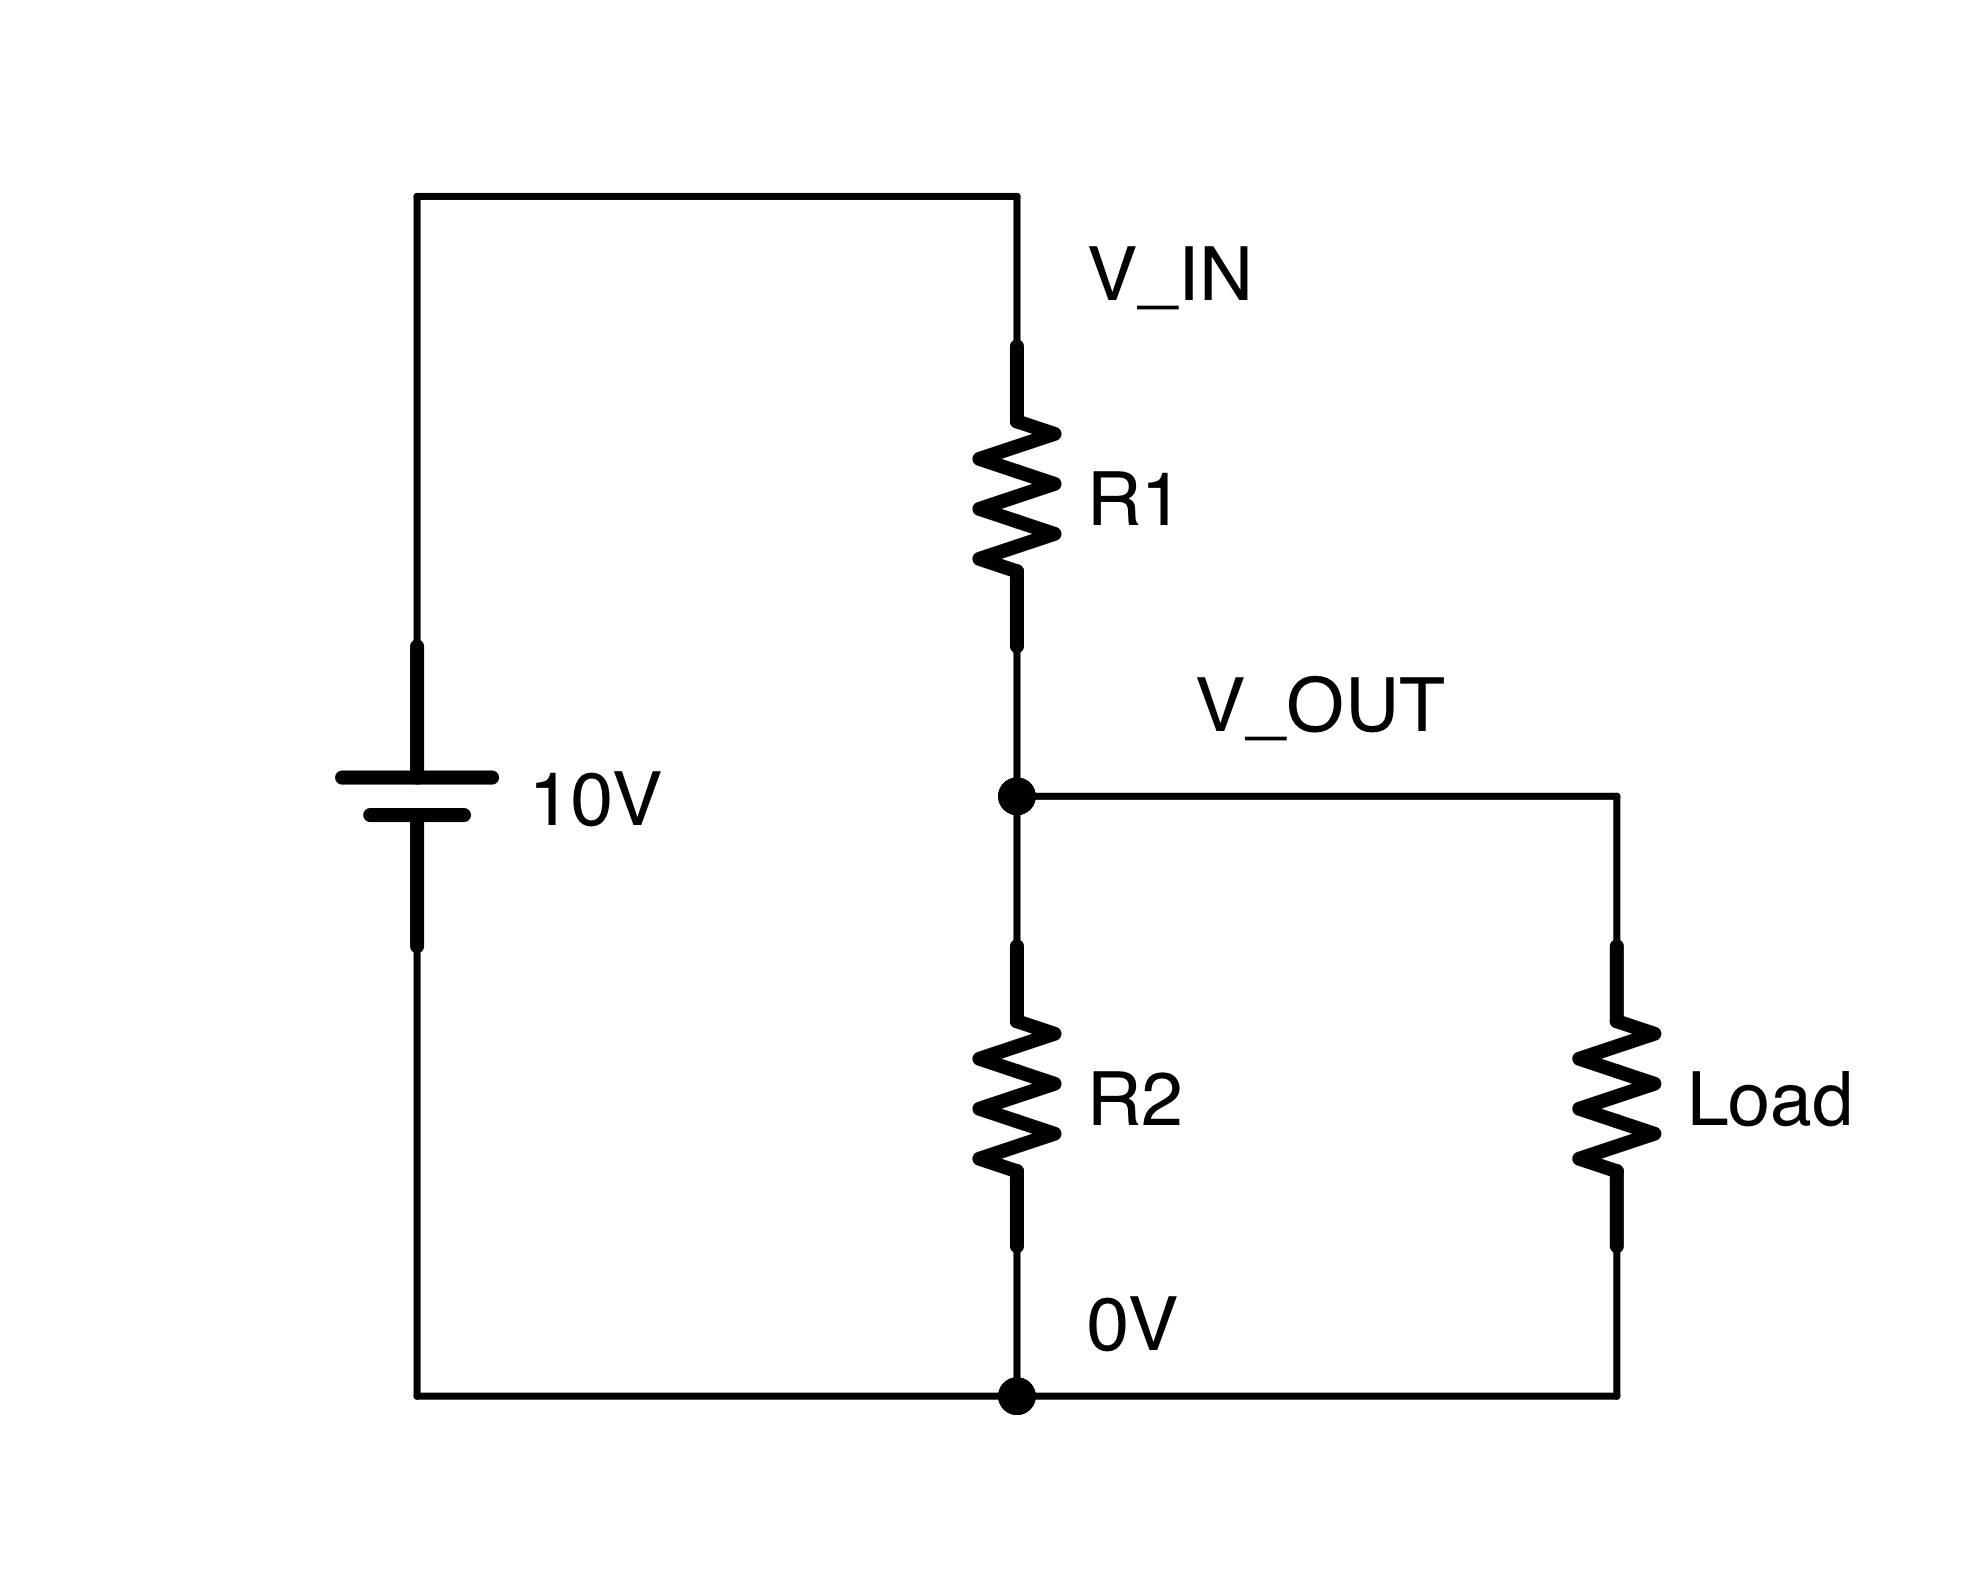
\includegraphics[width=\columnwidth]{ExVoltageDivider.png}
To achieve the required design, we need $R_1$ to be $428.57\myohm$ and $R_2$ to be $1,000\myohm$.}
\explanation{To create a voltage divider, we have to divide voltages between two resistors, with the output going out from between them.
Equation~\ref{eqVoltageDivision} shows us what the calculation looks like:
$$ V_{OUT} = V_{IN} * \frac{R_2}{R_1 + R_2} $$
Now, this equation only tells us about the ratio of the resistors, not what their specific value is.
For an equation for specific values for the resistors, we need to look at Equations~\ref{eqVDIVR2Eq} and~\ref{eqVDIVR1Eq}.
Equation~\ref{eqVDIVR2Eq} says:
\begin{align*}
R_2 &= R_L / 10 \\
    &= 10,000 / 10 \\
    &= 1,000\myohm
\end{align*}
Equation~\ref{eqVDIVR1Eq} says:
\begin{align*}
R_1 &= \frac{R_2 * (V_{IN} - V_{OUT})}{V_{OUT}} \\
    &= \frac{1,000 * (10 - 7)}{10} \\
    &= \frac{3,000}{7} \\
    &= 428.57\myohm
\end{align*}
Therefore, $R_1$ needs to be about $428.57\myohm$ and $R_2$ needs to be about $1,000\myohm$.
In reality, we would probably find a resistor that is close to $429\myohm$ even if it isn't exact.
Even a $400\myohm$ resistor would give a voltage within a few percent of the desired value.
}
\item 
\question{Given a $3\myvolt$ battery source, design a voltage divider that will output $1.5\myvolt$ to a load that has a resistance of $1\mykohm$.}
\solution{For this voltage divider, both $R_1$ and $R_2$ will be $100\myohm$.}
\explanation{Using the same equations as before, we can easily design a voltage divider. $R_2$ is determined by:
\begin{align*}
R_2 &= R_L / 10 \\
    &= 1,000 / 10 \\
    &= 100\myohm
\end{align*}
$R_1$ is determined by:
\begin{align*}
R_1 &= \frac{R_2 * (V_{IN} - V_{OUT})}{V_{OUT}} \\
    &= \frac{100 * (3 - 1.5)}{1.5} \\
    &= \frac{150}{1.5} \\
    &= 100\myohm
\end{align*}
Therefore, both $R_1$ and $R_2$ will be $100\myohm$.
}
\item 
\question{In Figure~\ref{figPullUpResistorBasic}, how much current is going through the circuit when the switch is open?  How much when it is closed?  You can assume that the LED is a red LED.}
\solution{The circuit uses $7.2\mymamp$ of current when the switch is open and $9\mymamp$ when the switch is closed.}
\explanation{When the switch is open, the current passes through \emph{both} the resistor and the LED.
Therefore, we have to account for the voltage drop of the LED itself as well as the resistance.
The starting voltage is $9\myvolt$ and a red LED will give a voltage drop of $1.8\myvolt$.
Therefore, the remaining voltage through the resistor will be $9 - 1.8 = 7.2\myvolt$.
Using Ohm's Law, we can find out the current flow:
\begin{align*}
I &= V / R \\
  &= 7.2 / 1,000 \\
  &= 0.0072\myamp = 7.2\mymamp
\end{align*}
Therefore, when the switch is open, the circuit consumes $7.2\mymamp$.
When it is closed, the current does \emph{not} flow through the LED.
The reason is that since there is a direct connection between the resistor and the ground, then the resistor \emph{must} be at a zero-volt state at the end of it.
Therefore, there is no voltage remaining to push through the LED.

Therefore, the entire $9\myvolt$ is flowing across the resistor.
This means that the calculation for Ohm's Law is as follows:
\begin{align*}
I &= V / R \\
  &= 9 / 1,000 \\
  &= 0.009 \myamp = 9\mymamp
\end{align*}
Therefore, when the switch is closed, the circuit uses $9\mymamp$ of current.
}
\item 
\question{How would you modify the circuit in Figure~\ref{figPullUpResistorBasic} to keep the maximum current in the circuit under $2\mymamp$?  Draw the full circuit out yourself.}
\solution{The full circuit should look like the below drawing:
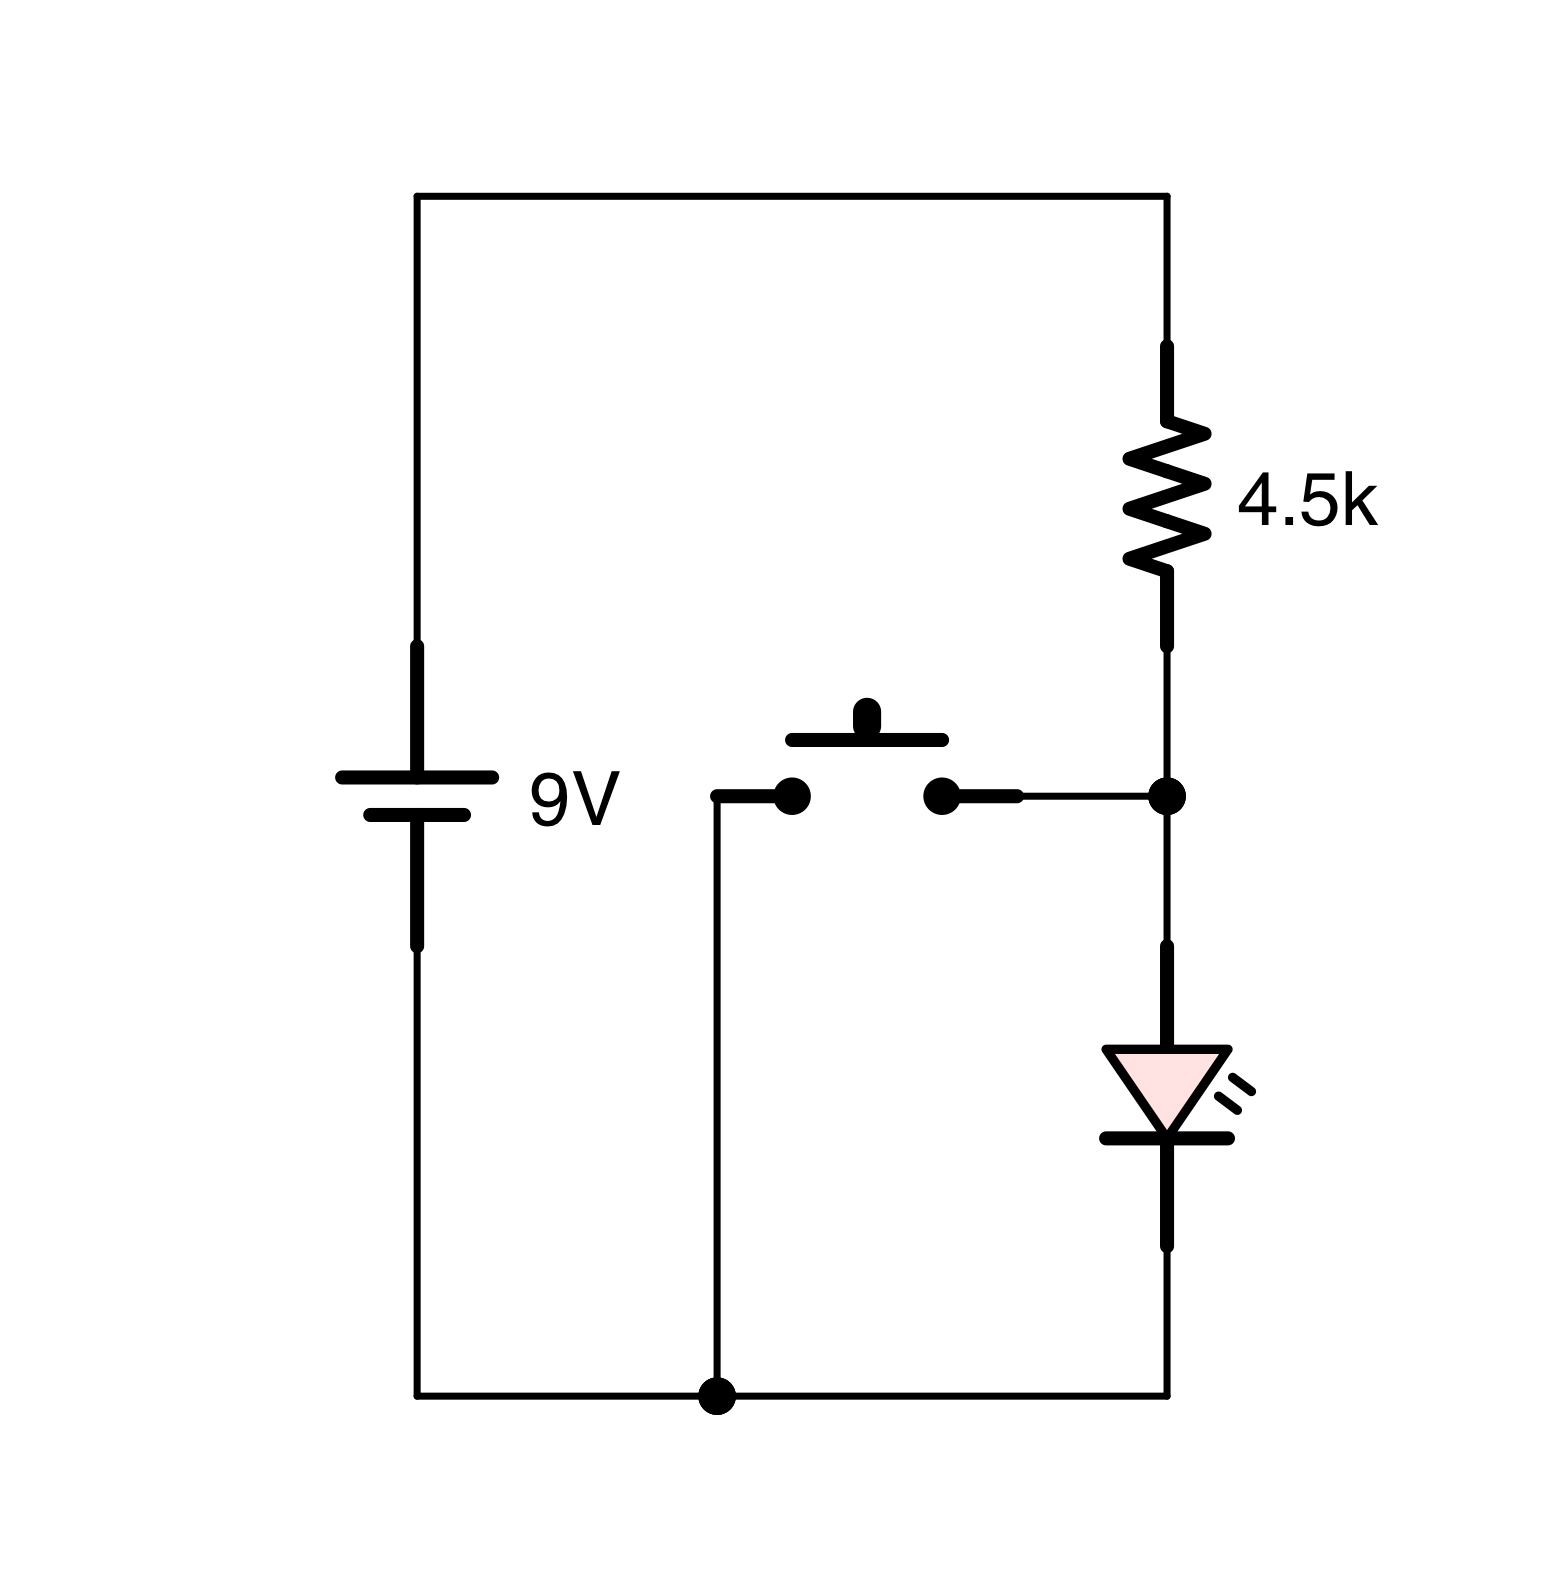
\includegraphics[width=\columnwidth]{ExPullUpResistorBasic.png}
}
\explanation{As we saw in the previous question, the circuit actually uses \emph{more} current when the switch is closed than when it is open.
Therefore, if we want to max sure the current never goes over $2\mymamp$ ($0.002\mymamp$), then we should design for that when the circuit is closed.
Therefore, using Ohm's Law, we can solve for the needed resistance like this:
\begin{align*}
R &= V / I \\
  &= 9 / 0.002 \\
  &= 4,500\myohm
\end{align*}
The drawn circuit should be identical to Figure~\ref{figPullUpResistorBasic} but with a $4,500\myohm$ resistor.
}
\item 
\question{Build the circuit you designed in the previous question.  If you do not have the right resistor values, use the closest ones you have.}
\solution{This is a project-building exercise.  The solution is correct if pushing the button turns off the light.  The one potential problem is if pushing the button creates a short circuit.  If this happens the project will get hot quickly.}
\end{enumerate}


\chapter{Understanding Power}


\begin{enumerate}
\item If I have 50 joules of energy, what is the maximum amount of work I could possibly do with that amount of energy?
\item If I am using up 10 joules of energy each second, how many watts am I using up?
\item If I convert 30 watts of mechanical power into electrical power with 50\% efficiency, how many watts of electrical power are delivered?
\item If I have a circuit powered by a $9\myvolt$ battery that uses $0.125\myamp$, how many watts does that circuit use?
\item If a resistor has a $2\myvolt$ drop with a $0.03\myamp$ current, how much power is the resistor dissipating?
\item If a resistor has a $3\myvolt$ drop with a $12\mymamp$ current, how much power is the resistor dissipating?
\item If a $700\myohm$ resistor has a $5\myvolt$ drop, how much power is the resistor dissipating?
\item If a $500\myohm$ resistor has $20\mymamp$ flowing through it, how much power is the resistor dissipating?
\item In the circuit below, calculate the voltage drop, current, and power dissipation of every component (except the battery). \\ 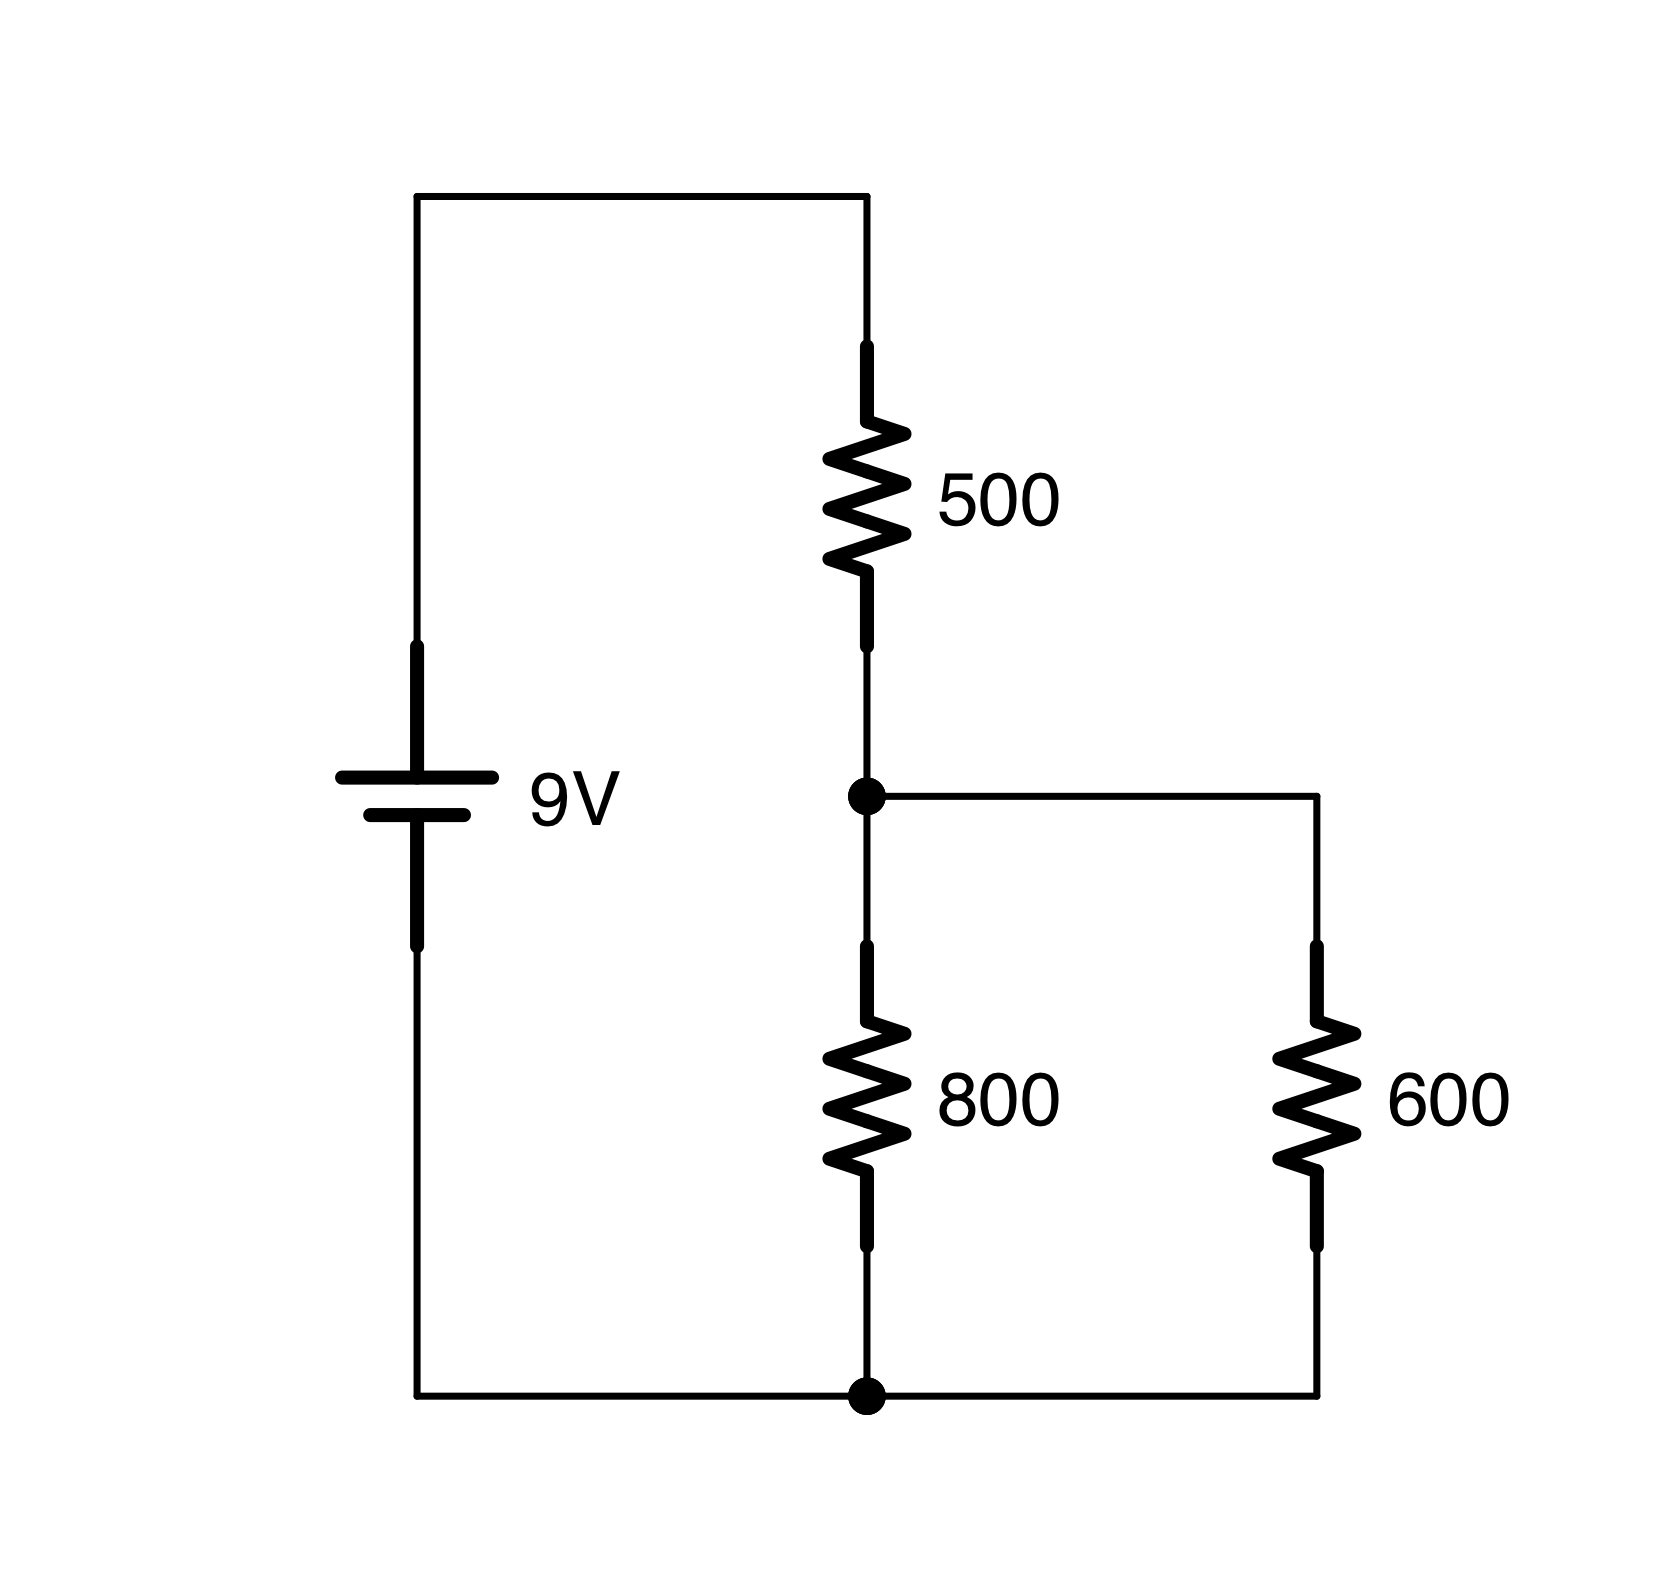
\includegraphics[scale=0.08]{ExampleForPowerDissipation.png}
\end{enumerate}


\chapter{Integrated Circuits and Resistive Sensors}


\begin{enumerate}
\item  Calculate the amount of current flowing through each element of the circuit in Figure~\ref{figSimpleComparatorCircuit}.  You can presume that the LM393 uses about $1\mymamp$ for its own operation, and that the LED is a red, $1.8\myvolt$ LED.  What is the total amount of current used by the circuit?
\item Take the circuit in Figure~\ref{figSimpleComparatorCircuit} and swap which voltage divider is attached to \icode{1IN+} and \icode{1IN-}.  Now calculate the total amount of current used by this circuit.
\item The Spectra Flex Sensor is a resistive sensor that changes its resistance when bent.  When it is straight, it has a resistance of $10\mykohm$.  When it is bent, it has resistances of $60\mykohm$ and above.  Draw a circuit that turns on an LED when the resistor is bent.  You may invent your own symbol for the flex sensor.
\item Build the circuit in Figures~\ref{figDarknessSensorCircuit} and~\ref{figDarknessSensorBreadboard}. 
\item If you wanted to wait until the room was even darker before the LED went on, how would you change the circuit?
\end{enumerate}


\chapter{Using Logic ICs}


\begin{enumerate}
\item 
\question{Draw the circuit in Figure~\ref{figLogicGateExample} yourself.  Identify the function of each resistor.}
\solution{
The circuit is repeated below:
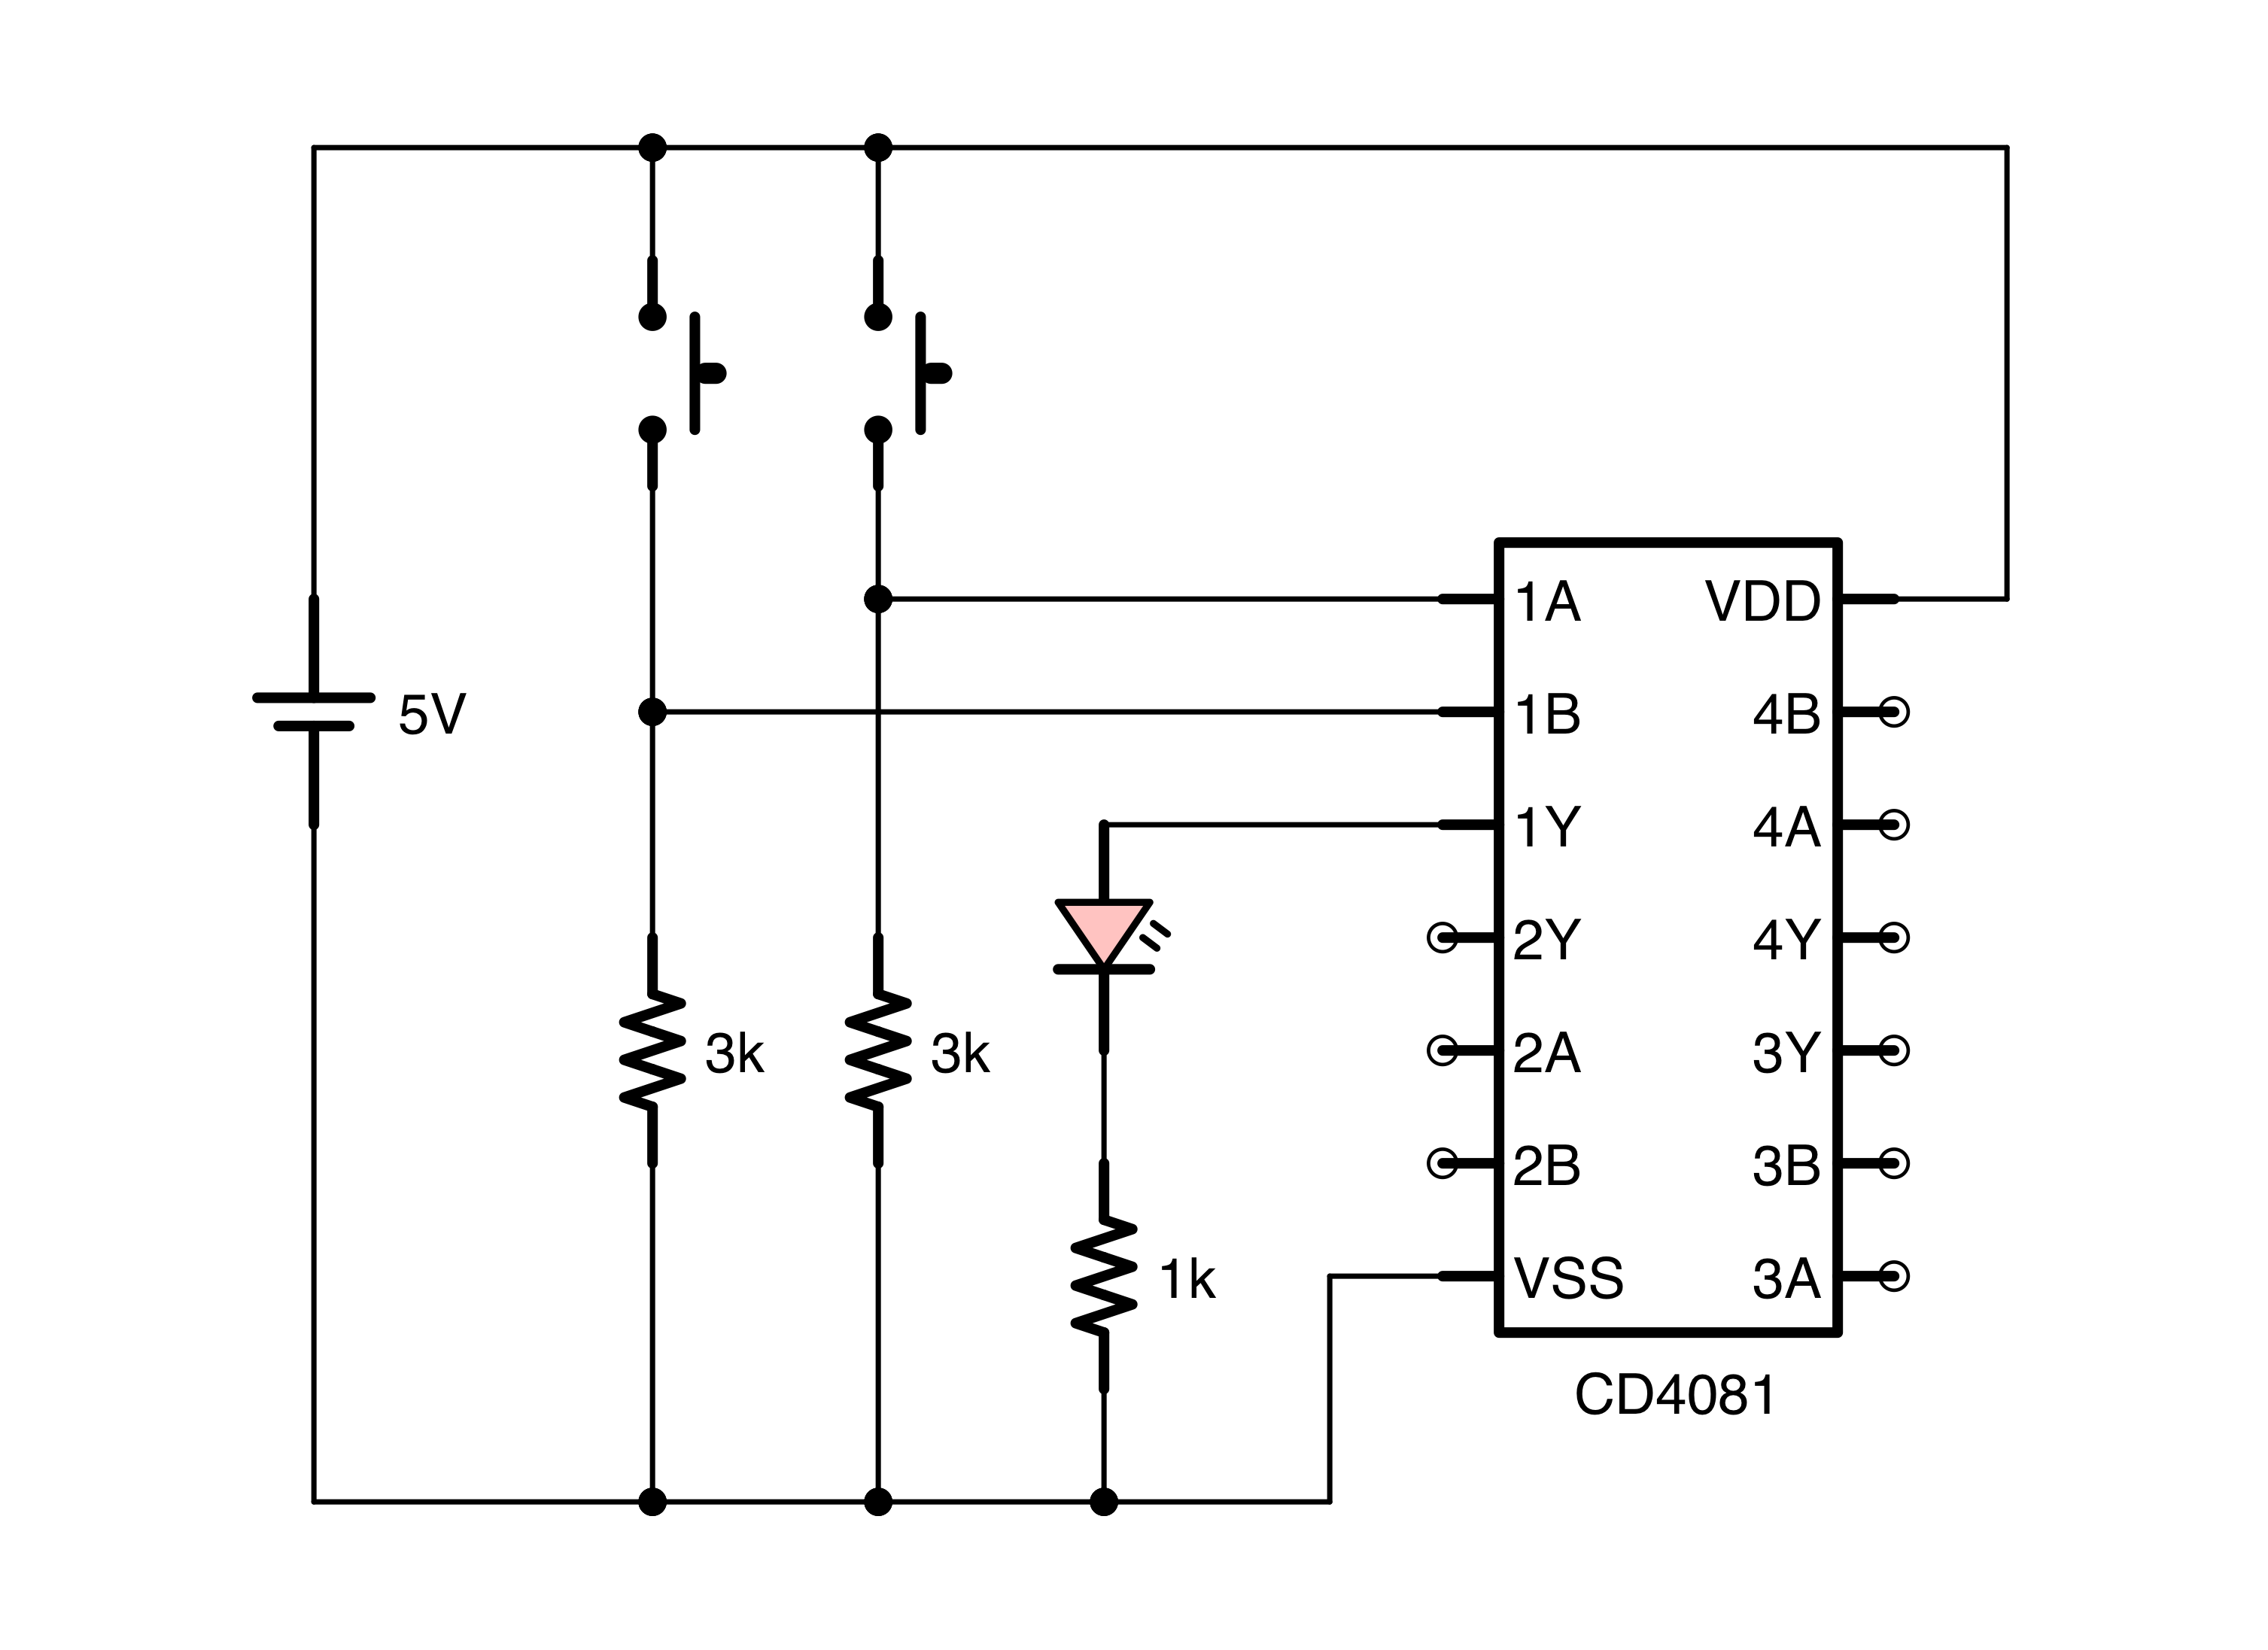
\includegraphics[width=\columnwidth]{LogicGateExample.png}

The 3k resistors are pull-down resistors.  The 1k resistor is a current-limiting resistor for the LED.
}
\item 
\question{Build the circuit in Figure~\ref{figLogicGateExample} (don't forget that the power source should be $5\myvolt$).}
\solution{When built, the circuit should only light up the LED when \emph{both} the buttons are pushed down.}
\item 
\question{If you assume that a negligible amount of current flows through the inputs of the AND gate, and that the output functions as a $5\myvolt$ voltage source (and the LED is red), how much current flows through each resistor when all of the buttons are pressed?  What, then, is the total current used by the circuit if you ignore the logic gate?}
\solution{The pull-down resistors each have $1.67\myamp$ of current, and the current-limiting resistor has $3.2\mymamp$ of current.  Therefore, the total current is $6.54\mymamp$.}
\explanation{When a button is pressed, there is a $3,000\myohm$ pull-down resistor connecting the power to ground.
Therefore, we can use Ohm's Law to find the current usage:
\begin{align*} 
I &= V / R \\
  &= 5 / 3,000 \\
  &= 0.00167\myamp = 1.67\mymamp
\end{align*}
Therefore, \emph{each} of the button circuits are using this amount of current.

Then, when both the inputs are positive, the output goes to $5\myvolt$.
This is dropped $1.8\myvolt$ by the red LED, leaving $3.2\myvolt$ for the resistor.
Therefore, the current going through the resistor is:
\begin{align*}
I &= V / R \\
  &= 3.2 / 1,000 \\
  &= 0.0032\myamp = 3.2\mymamp
\end{align*}
Therefore, the total amount of current in this circuit is $1.67 + 1.67 + 3.2 = 6.54\mymamp$.
}
\item 
\question{Measure the actual current that flows through each resistor.  If you are having trouble pushing the buttons while you measure the current, just replace the buttons with wires for this test.}
\solution{Your currents should roughly match the answers to the previous question.}
\item 
\question{Measure the current that it used by the AND gate itself.  You can do this by measuring the supply current of the AND gate.  Measure it both when its output is true and false.}
\solution{This measurement will vary depending on the brand of AND gate you are using.  However, usually it is less than $1\mymamp$ when the output is off.  It should increase by about the output current ($3.2\mymamp$) when the output is on.}
% FIXME - stopped adding solutions here.
\item 
\question{Draw a schematic of a circuit that has two buttons (B1 and B2) which light up an LED if either button is pressed.  Use the logic gate shapes for the schematic.}
\item 
\question{Draw a schematic of a circuit that has two buttons (B1 and B2) which light up an LED if neither button is pressed.  Use the logic gate shapes for the schematic.}
\item 
\question{Draw a schematic of a circuit that has four buttons (B1--B4) which light up an LED if either B1 and B2 are pressed or if B3 and B4 are pressed.  Use the logic gate shapes for the schematic.}
\item 
\question{Look at the construction of the different gates from NAND gates in Figure~\ref{figNANDLogic}.  Copy down the OR gate construction four times, and trace how the output is generated for each possible set of inputs (true/true, true/false, false/true, false/false).  Show the inputs and outputs on each NAND gate.  Compare the outputs to the truth table for the OR function in Figure~\ref{figTruthTable}.}
\item 
\question{Take the circuit in Figure~\ref{figLogicGateExample} and draw a schematic to use pull-up resistors on the inputs rather than pull-down resistors.  How will this change the behavior of the circuit?}
\item 
\question{Let's say that we want to create a door buzzer so that someone outside a door can push a button to be let in.  However, the person inside also wants a switch to be able to disable the buzzer.  The buzzer can be thought of as a simple device that buzzes when any positive voltage is applied.  Draw a circuit diagram of this setup using logic gates.  The buzzer can be drawn as a resistor labelled ``buzzer'' (don't forget to connect the other side to ground!).}
\end{enumerate}


\chapter{Introduction to Microcontrollers}


\begin{enumerate}
\item 
\question{Practice modifying and uploading the Blink program to the Arduino Uno.  Change the numbers given to \icode{delay} to different values, and see how that affects the operation of the program.}
\solution{Changing the value for the delay should cause the light to noticeably blink at different rates.}
\item 
\question{The ATmega328/P is only one of many different microcontrollers available in the AVR family.  Research online to find one or two other AVR chips and what different features they have.}
\solution{There are many different types of AVR chips.  Some of the others include the ATTiny series, the ATmega series, and the XMEGA.  These chips generally differ by available memory, number of pins, and add-on subsystems.}
\item 
\question{The AVR family is only one of many microcontroller families.  Research one or two other microcontroller families and look at what features are claimed for each.  Examples of other microcontroller families include: PIC, STM32, MSP432, and the Intel Quark.}
\solution{This is an open-ended question.  Features that would be interesting to focus on are power consumption, working voltage, available memory, ease of programming, extra features, size, and other characteristics.}
\item 
\question{Go to the \icode{arduino.cc} website and look at the different types of Arduinos that are available.  What makes them different?  Why might you choose one for a project over another?}
\solution{While Arduino continually comes out with new variants, some popular variants include the Arduino Uno, the Leonardo, the 101, the Nano, the MKR series, the M0, the Due, and others.  These differ from each other based on size, the microcontroller family (AVR, Intel, etc.), the specific microcontroller (which varies based on RAM, speed, power consumption, extra features, etc.), and the extras packed onto the board.  The MKR series, for instance, combines the microcontroller with different kinds of networking features.  Also, some of them vary by the working voltages used as well.  Some variants such as the Lilypad are geared towards wearable devices.}
\end{enumerate}


\chapter{Building Projects with Arduino}

\begin{enumerate}
\item 
\question{Which Arduino pin do you use when supplying an unregulated voltage (i.e., a voltage above the $5\myvolt$ that the Arduino runs at)?}
\solution{The $V_{IN}$ pin is used to provide an unregulated voltage to the Arduino.}
\question{What Arduino pins would you use to extract power out from an Arduino connected to a power supply?}
\solution{You would use the $5\myvolt$ pin for a regulated five volt output, and the $GND$ pin for ground.}
\question{What is the voltage of an output pin set to HIGH?}
\solution{An output pin set to HIGH puts out $5\myvolt$.}
\question{What is the maximum current that should be sourced by any particular Arduino pin?}
\solution{Each output pin should only have up to $20\mymamp$ of current coming out of it.}
\question{If you have a red LED attached to an Arduino output pin, what is the minimum size of resistor that you need?}
\solution{$160\myohm$}
\explanation{Since each output pin can only output $20\mymamp$ of current, we can use Ohm's Law to figure out the minimum size of resistor.
The red LED will eat up $1.8\myvolt$ of voltage. 
That leave $5 - 1.8 = 3.2\myvolt$ remaining.
Therefore, Ohm's Law states:
\begin{align*}
R &= V / I \\
  &= 3.2 / 0.02 \\
  &= 160\myohm
\end{align*}
Therefore, the resistor needs to be at least $160\myohm$.
}
\question{If an Arduino input pin is completely disconnected from a circuit, what state does the Arduino read it as?}
\solution{If a pin is completely disconnected from a circuit, it could read any value---either HIGH or LOW.}
\question{How much current does an Arduino input use?}
\solution{Arduino inputs can be thought of as mere voltage sensors, not using up any serious amount of current.}
\question{What is the best way to wire a button to an Arduino?}
\solution{Buttons should be wired to Arduinos with pull-down (or pull-up) resistors, in order to make sure that the input pin is always physically connected to the circuit, and therefore has a valid value.}
\question{What is an advantage of storing a program in a microcontroller even if the logic could be built directly in hardware?}
\solution{Storing a program in a microcontroller allows \emph{changes} in logic to be performed without remanufacturing.  Additionally, the microcontroller can often be cheaper (and smaller) than the device built without them.}
\end{enumerate}


\chapter{Analog Input and Output on an Arduino}

\begin{enumerate}
\item \fixme{Add exercises here}
\end{enumerate}


\chapter{Capacitors}


\begin{enumerate}
\item Convert $23\myf$ to microfarads.
\item Convert $15\myuf$ to farads.
\item Convert $0.0002\myf$ to microfarads.
\item Convert $0.0030\myuf$ to farads.
\item If a voltage of $6\myvolt$ is applied to a $55\myuf$ capacitor, how much charge would it store?
\item If a voltage of $2\myvolt$ is applied to a $13\mypf$ capacitor, how much charge would it store?
\item If a $132\myuf$ capacitor is holding $0.02\textrm{ coulombs}$ of charge, how many volts will it produce when it discharges?
\item if a $600\mypf$ capacitor is holding $0.03\textrm{ coulombs}$ of charge, how many volts will it produce when it discharges?
\item If a $121\myuf$ capacitor is connected to a battery.  After some fluctuation, the capacitor has $0.00089\textrm{ coulombs}$ of charge stored in it and the battery is reading $8.9\myvolt$.  Is the capacitor going to be charging or discharging at this point?
\end{enumerate}


\chapter{Capacitors as Timers}


\begin{enumerate}
\item If I have an RC circuit with a resistor of $10\myohm$ and a capacitor of $2\myf$, what is the RC time constant of this circuit?
\item In the previous question, how many seconds does it take to charge my capacitor to approximately 50\% of supply voltage?
\item If I have an RC circuit with a resistor of $30,000\myohm$ and a capacitor of $0.001\myf$, what is the RC time constant of this circuit?
\item In the previous question, what percentage of the way is the capacitor charged after 60 seconds?
\item If I have an RC circuit with a resistor of $25\mykohm$ and a capacitor of $20\myuf$, what is the RC time constant of this circuit?
\item Give a resistor and capacitor combination that will yield an RC time constant of 0.25 seconds.
\item Reconfigure the circuit in Figure~\ref{figSimpleTimerCircuit} to wait for 3 seconds.  Draw the whole circuit.
\item Redraw the previous circuit, and circle each basic circuit pattern and label it.
\end{enumerate}


\chapter{Introduction to Oscillator Circuits}


\begin{enumerate}
\item 
\question{Take a look at the circuit in Figure~\ref{figSimple555Oscillator} (this will be used as the basis for the problems in this section).   Copy this circuit to a piece of paper.  Draw a line in one color showing how the current flows in the main circuit as it charges the capacitor.  With a different color, draw a line showing how current flows as the capacitor discharges.  Use arrows to indicate current direction.  You can ignore the ``Output'' and ``Control'' sections of the circuit for this problem.}
\solution{The lines should be drawn as follows:\newline
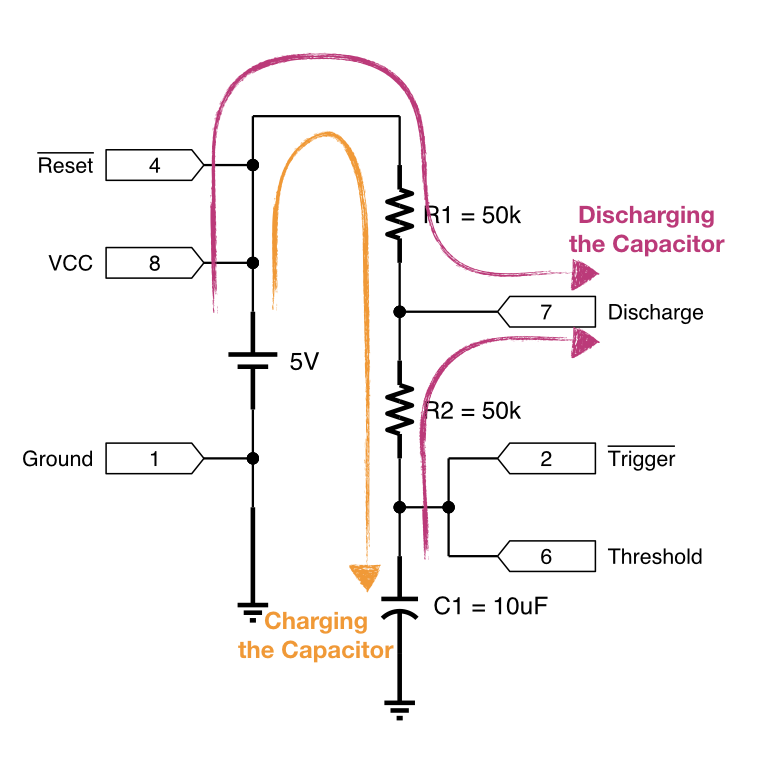
\includegraphics[width=0.8\columnwidth]{ExOscillatorChargeDischarge.png}
}
\explanation{
During the charging phase, current flows from the positive all the way into the capacitor.
This is shown with the line that is on the interior of the circuit.
During the discharge phase, Pin~7 goes low, and therefore current flows into Pin~7 from \emph{both}
the power supply \emph{and} from the capacitor.
}
\item 
\question{Why is R1 important?  What would happen if we just replaced it with a wire?}
\solution{During the discharge phase, R1 acts as a current-limiting resistor.  It would create a short-circuit from power to ground if it was just a wire.}
\explanation{Remember, there is no intelligence in a circuit.
The power supply only knows how to supply power.
Therefore, during the discharge phase, the power supply \emph{will continue to supply power just as before}.
When Pin~7 goes to zero volts, not only does the charge from the capacitor start to flow in that direction, but also the power from the supply.
If there is no resistor here, then it becomes a short-circuit from supply to ground.
Additionally, since this power is entirely wasted, R1 also limits the amount of waste that occurs during the discharge phase.
}
\item 
\question{Why are there two different pins on the NE555 connected to the capacitor?  What type of circuit (that we have discussed in this book) do you think they are connected to inside the chip?}
\solution{One compares for voltage \emph{above} a certain level, and the other compares for voltage \emph{below} a certain level.  Since they are checking for voltage, they are probably voltage comparator circuits.}
\explanation{The NE555, in its standard configuration, allows the capacitor to charge until it is two thirds full, and then discharges it until it is only one third full.
It has to detect for each of these conditions.
Therefore, it has two separate sensing inputs, one for each condition.  
$Threshold$ watches for the high voltage (and switches it from ``charge'' to ``discharge'' when it goes over), and $\overline{Trigger}$ watches for the low voltage (and switches it from ``discharge'' to ``charge'' when it goes under).
Since it is watching voltage levels, it is likely using a voltage comparator in the chip to measure these voltages.
}
\item 
\question{Why is the charging time of the NE555 always at least a little longer than the discharging time?}
\solution{The circuit uses both R1 and R2 to charge, but \emph{only} uses R2 to discharge.  Therefore, the resistance for discharging will always be less than the resistance for charging.}
\item 
\question{Why does the NE555 stay in the on state a little longer when the circuit is first turned on?}
\solution{Generally, the NE555 oscillates between filling and discharging the capacitor from one third to two-thirds full.  When first turned on, the capacitor will (presumably) be \emph{fully} discharged, so it will take some amount of time for that first charge cycle to occur, because it is charging from zero instead of from one third full.}
\item 
\question{Let's say that we wanted our circuit to be on for $2\mysec$ and off for $1\mysec$.  Keeping the same capacitor, what values should we use for R1 and R2 to accomplish that?}
\solution{R1 would be $144300.2\myohm$ and R2 would be $144300.1\myohm$.  In terms of standard components, using a $150\mykohm$ resistor for each one would be sufficient.}
\explanation{Since the discharge phase (when the output is off) only uses one resistor (R2) we will beging considering the discharge phase.
The total time is $1\mysec$.
Since we are using a NE555 timer, this time will cover $0.693$ time constants.
The time constant is given by the resistance multiplied by the capacitance.
Since the capacitor is a $10\myuf$ capacitor, the full equation is:
\begin{align*}
R \cdot 0.00001 \cdot 0.693 &= 1 \\
R &= \frac{1}{0.00001 \cdot 0.693} \\
R &\approx 144300.1
\end{align*}
Therefore, R2 will be approximately $144300.1\myohm$.
We now do a similar operation to find R1.  
However, the ``on'' phase of the oscillation will utilize both R1 and R2, and will take two seconds.
Therefore, we can solve for R1 as follows:
\begin{align*}
0.00001 \cdot (144300.1 + R) &\cdot 0.693 = 2 \\
144300.1 + R &= \frac{2}{0.00001 \cdot 0.693} \\
R &= \frac{2}{0.00001 \cdot 0.693} - 144300.1 \\
R &\approx 144300.2 
\end{align*}
So R1 will be approximately $144300.2\myohm$.

Resistors are not actually available in these values.
Therefore, you would likely choose a $150\mykohm$ resistor for each of these.
}
\item 
\question{Let's say that we wanted our circuit to be on for $10\mysec$ and off for $3\mysec$.  Keeping the same capacitor, what values should we use for R1 and R2 to accomplish that?}
\item 
\question{The factory called and said that they were out of the capacitor we wanted for the circuit, and instead only had a $23\myuf$ capacitor that we could use.  Recalculate the previous problem using this new capacitor value.}
\item 
\question{How much current is our output sourcing from the chip?}
\item 
\question{When the chip first turns on (and thus the capacitor is empty and at $0\myvolt$) how much current is the RC circuit using?}
\end{enumerate}

% FIXME - might have a problem where people draw the pinout of the 555
% FIXME - might have a problem where they draw a circuit and then circle different part


\chapter{Producing Sound with Oscillations}


\begin{enumerate}
\item Why is the input voltage signal to the 555 timer smooth, but the output is square?
\item Will increasing the resistance of R1 and R2 make the pitch higher or lower?
\item Can you think of a way to modify the circuit so that the pitch of the sound can be adjusted while the circuit is on? 
\item Given the circuit in Figure~\ref{figSimpleToneGenerator}, what power would be delivered to your headphones if you were using an $8\myohm$ speaker instead of the $16\myohm$ speaker?  What about a $100\myohm$ speaker?
\item The frequency of the A note above middle-C on the piano is $440\myhz$.  Design a modification to this circuit that will yield this frequency.
\item The output of the 555 is $1.7\myvolt$ less than the power supply used.  What is the effect on the wattage to the headphones if we change the power supply to be a $9\myvolt$ power supply?
\end{enumerate}


\chapter{Inductors}


\begin{enumerate}
\item 
\question{If I want a circuit to block DC current but allow AC current, should I use an inductor or a capacitor?}
\solution{Capacitor}
\explanation{Capacitors allow AC current but block DC current.}
\item 
\question{If I want a circuit to allow DC current but block AC current, should I use an inductor or a capacitor?}
\solution{Inductor}
\explanation{Inductors allow DC current but block AC current.}
\item 
\question{Why are inductors used so much in systems that interact with the outside world?}
\solution{Inductors create a magnetic field which can be used to move other components.}
\item 
\question{Why does inductive kick happen?}
\solution{In an inductor, the magnetic field is maintained through current flow through the inductor.  If the current decreases, the magnetic field cannot be maintained, and the flux is converted to a voltage.  A sudden decrease in current will cause an equally sudden build-up in voltage.  This is the inductive kick.}
\item 
\question{Draw a schematic of an inductor where the positive side of the inductor has a switch and the negative side is connected to an LED and a resistor.  Add in a snubber diode to protect the LED from the effect of turning off the switch.}
\solution{\newline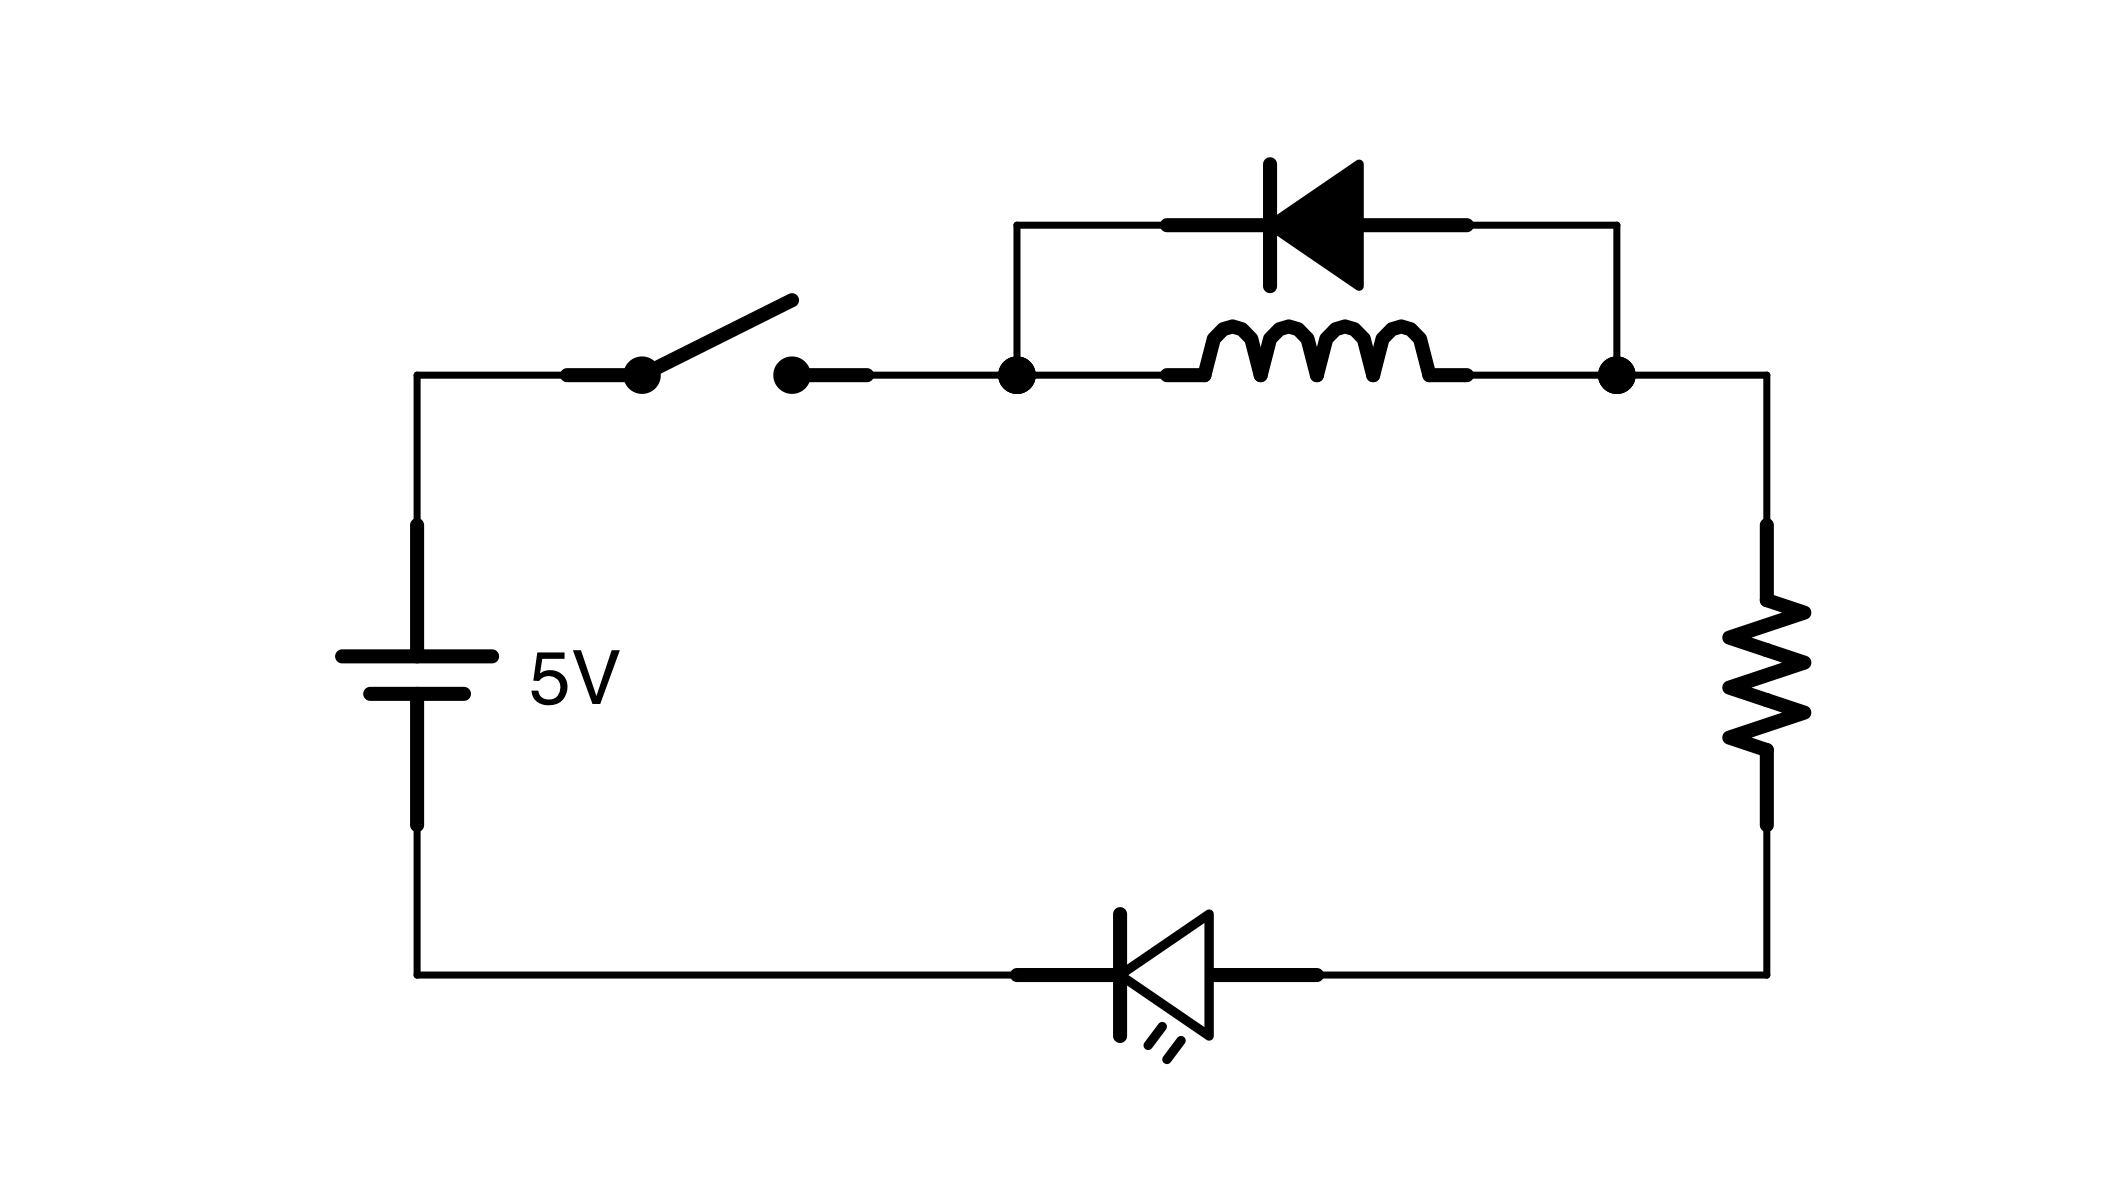
\includegraphics[width=0.7\columnwidth]{SolutionSnubberDiode.png}}
\item
\question{What is the purpose of the snubber diode?}
\solution{The snubber diode reduces the effect of the inductive kick by giving the current a pathway back through the inductor.
This allows generated voltages/currents to be bled off slowly throught the inductor itself.}
\item 
\question{If I have an inductor that is $5\myhy$ and has a steady current going through it of $2\myamp$, what is the size of the magnetic flux in the inductor's magnetic field?}
\solution{$10$ webers}
\explanation{The equation governing the behavior of an inductor is given by Equation~\ref{eqinductance}, $\phi = L \cdot I$, where $L$ is given in henries and $I$ is in amperes.
Therefore, since the units match, we can calculate as follows:
\begin{align*}
\phi &= L \cdot I \\
 &= 5 \cdot 2 \\
 &= 10
\end{align*}
Therefore, the inductor is holding $10$ webers of flux.
}
\item 
\question{If I have an inductor that is $7\myuhy$ and has a steady current going through it of $3\mymamp$, what is the size of the magnetic flux in the inductor's magnetic field?}
\solution{$0.000000021$ webers}
\explanation{The equation for flux is $\phi = L \cdot I$, where $L$  is in henries and $I$ is in amperes.
Therefore, we need to convert into proper units to use the equation.
Since $1\myuhy = 0.000001\myhy$, $7\myuhy = 0.000007\myhy$.
Since $1\mymamp = 0.001\myamp$, $3\mymamp = 0.003\myamp$.
Therefore, the equation becomes:
\begin{align*}
\phi &= L \cdot I \\
 &= 0.000007 \cdot 0.03 \\
 &=0.000000021
\end{align*}
Therefore, the magnetic field has a flux of $0.000000021$ webers.
}
\item 
\question{If I have a $4\myhy$ inductor with $0.3\mywb$ of flux in its magnetic field, how much current is flowing through it?}
\solution{$0.075\myamp$ or $75\mymamp$}
\explanation{We will solve this problem by rearranging Equation~\ref{eqinductance} to solve for $I$:
\begin{align*}
\phi &= L \cdot I \\
I &= \frac{\phi}{L}
\end{align*}
Since the units are already correct, I can now just substitute and solve:
\begin{align*}
I &= \frac{\phi}{L} \\
 &= \frac{0.3}{4} \\
 &= 0.075
\end{align*}
Therefore, the current is $0.075\myamp$ or $75\mymamp$.
}
\item 
\question{If an inductor's magnetic field has $5\mywb$ of flux and it decreases to $3\mywb$ of flux over $2\mysec$, what is the average voltage produced over that timeframe?}
\solution{}
\explanation{Questions involving the \emph{change} of voltage and flux utilize Equation~\ref{eqlenz}, which states:
\begin{align*}
V_{\textrm{average}} = -\frac{\textrm{change in }\phi}{\textrm{change in time}}
\end{align*}
Since we start with $5\mywb$ of flux and end with $3\mywb$, therefore, we changed by $-2\mywb$.
Since this occurred across $2\mysec$, the resulting formula would be:
\begin{align*}
V_{\textrm{average}} &= -\frac{-2}{2} \\
  &= 1
\end{align*}
Therefore, the average voltage produced for that time period is $1\myvolt$.
}
\item 
\question{If an inductor's magnetic field has $1\myuwb$ of flux and it increases to $2\myuwb$ of flux over $0.4\mysec$, what is the average voltage produced over that timeframe?}
\solution{}
\explanation{Questions involving the \emph{change} of voltage and flux utilize Equation~\ref{eqlenz}.  To use this equation, first we have to convert units.
The standard conversion is $1\myuwb = 0.000001\mywb$.
Therefore, the equation becomes:
\begin{align*}
V_{\textrm{average}} &= -\frac{\textrm{change in }\phi}{\textrm{change in time}} \\
 &= -\frac{0.000001}{0.4} \\
 &= -0.0000025
\end{align*}
Therefore, the inductor will produce a negative voltage, averaging $-0.0000025\myvolt$ for the duration of the $0.4\mysec$.
}
\item 
\question{If the current flowing through a $3\myhy$ inductor drops from $7\mymamp$ to $1\mymamp$ over a period of $0.01\mysec$, what is the average voltage produced over that time period?}
\solution{$1.8\myvolt$}
\explanation{To solve this, you will need \emph{both} Equation~\ref{eqinductance} and Equation~\ref{eqlenz}.
Equation~\ref{eqlenz} requires a starting and an ending flux. 
However, we are not given the starting and ending flux, but rather the starting and ending current.
Equation~\ref{eqinductance} tells us how to relate current to the amount of flux.

First, we need to convert our units.
$7\mymamp = 0.007\myamp$ and $1\mymamp = 0.001\myamp$.
Let's begin by solving for the starting flux:
\begin{align*}
\phi &= L \cdot I \\
 &= 3 \cdot 0.007 \\
 &= 0.021
\end{align*}
So the starting flux is $0.021\mywb$.

Next, let's solve for the final flux:
\begin{align*}
\phi &= L \cdot I \\
 &= 3 \cdot 0.001 \\
 &= 0.003
\end{align*}
So, the final flux is $0.003\mywb$.
This means that the change in flux was $-0.018\mywb$ across $0.01\mysec$.
Therefore, the average voltage over that period can be found using Equation~\ref{eqlenz}:
\begin{align*}
V_{\textrm{average}} &= -\frac{\textrm{change in }\phi}{\textrm{change in time}} \\
 &= -\frac{-0.018}{0.01} \\
 &= 1.8
\end{align*}
Therefore, the average voltage produced by the decrease in current over that time period is $1.8\myvolt$.
}
\end{enumerate}


\chapter{Inductors and Capacitors in Circuits}


\begin{enumerate}
\item What is the time constant of a series circuit consisting of a $50\myohm$ resistor and a $2\myhy$ inductor?
\item What is the time constant of a series circuit consisting of a $10\myohm$ resistor and a $5\myuhy$ inductor?
\item If I have a $9\myvolt$ battery and I connect it to a series circuit consisting of a $1\mykohm$ resistor and a $23\myuhy$ inductor, how much time will it take before the current through the inductor reaches approximately 87\% of its maximum value?
\item If I have a $5\myvolt$ source and I connect it to a series circuit consisting of a $2\mykohm$ resistor and a $6\myuhy$ inductor, how much time will it take before the voltage across the inductor falls below $0.25\myvolt$.
\item If I have a circuit that has unwanted high-pitched noise, what component can I wire in series with the circuit to remove the noise?
\item If I have a circuit that has unwanted high-pitched noise, what component can I wire in parallel with the circuit to remove the noise?
\item What types of currents does an inductor (a) block and (b) allow?
\item What types of currents does a capacitor (a) block and (b) allow?
\item If I am building a radio, I need to allow through only very specific frequencies.  What component or combination of components would I use to do this?
\end{enumerate}



\chapter{Reactance and Impedance}


\begin{enumerate}
\item As the frequency of a signal goes up, how does that affect the reactance from a capacitor?  What about with an inductor?
\item As the frequency of a signal goes down, how does that affect the reactance from a capacitor?  What about with an inductor?
\item What is true about the relationship between the capacitative reactance and the inductive reactance at the resonant frequency?
\item Why is power not used up with reactance?
\item How are reactance and resistance combined to yield impedance?
\item Calculate the capacitative reactance of a $3\myf$ capacitor at $5\myhz$.
\item Calculate the capacitative reactance of a $20\myuf$ capacitor at $200\myhz$.
\item Calculate the inductive reactance of a $7\myhy$ inductor at $10\myhz$.
\item Calculate the inductive reactance of a $8\mymhy$ inductor at $152\myhz$.
\item Calculate the impedance of a circuit with a $200\myohm$ resistor in series with a $75\myuf$ capacitor with a signal of $345\myhz$.
\item Calculate the impedance of a circuit with a $310\myohm$ resistor in series with a $90\mynf$ capacitor with a signal of $800\myhz$.
\item Calculate the impedance of a circuit with no resistor and a $60\mymhy$ inductor with a signal of $89\myhz$.
\item Calculate the impedance of a circuit with a $50\myohm$ resistor in series with a $75\myuhy$ inductor with a signal of $255\myhz$.
\item If I have an AC circuit with an RMS voltage of $6\myvolt$ and an impedance of $1\mykohm$, what is the average (RMS) current of this circuit?
\item If I have an AC circuit, and I measure the AC voltage as $10\myvolt$ RMS, and I measure the AC current at $2\mymamp$ RMS, what is the impedance of this circuit?
\item If I have an $80\myhz$ AC circuit that has an $8\myvolt$ RMS voltage source in series with a $500\myohm$ resistor, a $5\myhy$ inductor, and a $200\mynf$ capacitor, what is the RMS current flowing in this circuit?
\item Calculate the impedance of a circuit with a $250\myohm$ resistor in series with a $87\myuhy$ inductor and a $104\myuf$ capacitor with a signal of $745\myhz$.
\item What is the resonant frequency of the circuit in the previous question?
\item What is the reactance of a circuit at its resonant frequency?
\item If I have a $10\myuf$ capacitor, what size inductor do I need to have a resonant frequency of $250\myhz$?
\end{enumerate}


\chapter{DC Motors}


\begin{enumerate}
\item If you wanted to prevent too much current from going through a motor, what should you use for this?
\item What happens to the RPM of a motor when I reduce the voltage to my motor?
\item What should be attached to a motor to protect the other parts of the circuit when a motor is shut-off?
\item List one reason why a series resistor should not be used with a motor.
\item If I was building a robot and wanted to control the angle of a robot's arm, what type of motor could I use?
\item If I was building a machine to place components into a precise position onto a board, what type of motor should I pick to achieve that precision?
\end{enumerate}


\chapter{Amplifying Power with Transistors}


Unless otherwise specified, assume that the transistor is a BJT NPN transistor and that the beta is stable.

\begin{enumerate}
\item If the base of a transistor is at $3\myvolt$ and the transistor is on, what will be the emitter voltage?
\item If the base of a transistor is at $45\myvolt$ and the emitter is on, what will be the emitter voltage?
\item If the base of a transistor is at $5\myvolt$ and the emitter, if conducting, would have to be at $4.5\myvolt$, is the transistor on or off?
\item If the base of a transistor is at $0.6\myvolt$ and the emitter is at ground, is the transistor on or off?
\item If the base of a transistor is at $0.4\myvolt$ and the emitter is at ground, is the transistor on or off?
\item If a transistor has a base current ($I_{BE}$) of $2\mymamp$ and the transistor has a beta of $55$, how much current is going through the collector ($I_{CE}$)?
\item In the previous problem, how much total current is coming out of the emitter?
\item If a transistor has a base current of $3\mymamp$ and the transistor has a beta of $200$, how much current is going through the collector?
\item If the base voltage is greater than the collector voltage, what does this mean for our transistor operation?
\item The output of your microcontroller is $3.3\myvolt$ and supports a maximum output current of $10\mymamp$.  Using Figure~\ref{figArduinoTransistorSwitchOnMotor} as a guide, design a circuit to control a motor that requires $80\mymamp$ to operate.  Assume that the transistor beta is 100.
\item Redesign the previous circuit so that it utilizes a stabilizing resistor on the emitter to prevent variations in the transistor beta.
\end{enumerate}


\chapter{Transistor Voltage Amplifiers}

\begin{enumerate}
\item What is the purpose of the resistor in the collector of a transistor amplifier?
\item What is the purpose of the resistor in the emitter of a transistor amplifier?
\item Why is there a bias voltage on the base of the transistor?  Why can't the signal just be connected in directly to the base?
\item Why is the signal coupled in through a capacitor?
\item Why does the single stage voltage amplifier discussed in this chapter invert its output?
\item If the output of the two-stage amplifier is coupled into a third stage, the signal current would swing $1.85\mymamp$ in either direction.  Design a third amplification stage which can handle this amount of current.
\end{enumerate}


\chapter{Examining Partial Circuits}

\begin{enumerate}
\item Why would we want to know what a circuit's \thev Equivalent circuit is?
\item What are the two components of a \thev Equivalent circuit?
\item Think about the two-stage amplifier that you built in Chapter~\ref{chapTransVoltageAmp}.  How would you go about finding the \thev Equivalent circuit as it is seen by the headphones?
\item Suppose I have a circuit where the output terminals have a $2\myvolt$ drop when it is an open circuit, and have $2\mymamp$ of current flowing through it when it is a short circuit.  Draw the \thev Equivalent circuit.
\item If I have a \thev Equivalent circuit of $4\myvolt$ with an impedance of $400\myohm$, what will be the voltage drop of the load if I attach a $2000\myohm$ resistor across the output?
\item If I have a \thev Equivalent circuit of $3\myvolt$ with an impedance of $100\myohm$, what will be the voltage drop, the current, and the power of the load if I attach headphones rated at $32\myohm$?
\item Calculate and draw the \thev Equivalent circuit of the circuit below: 
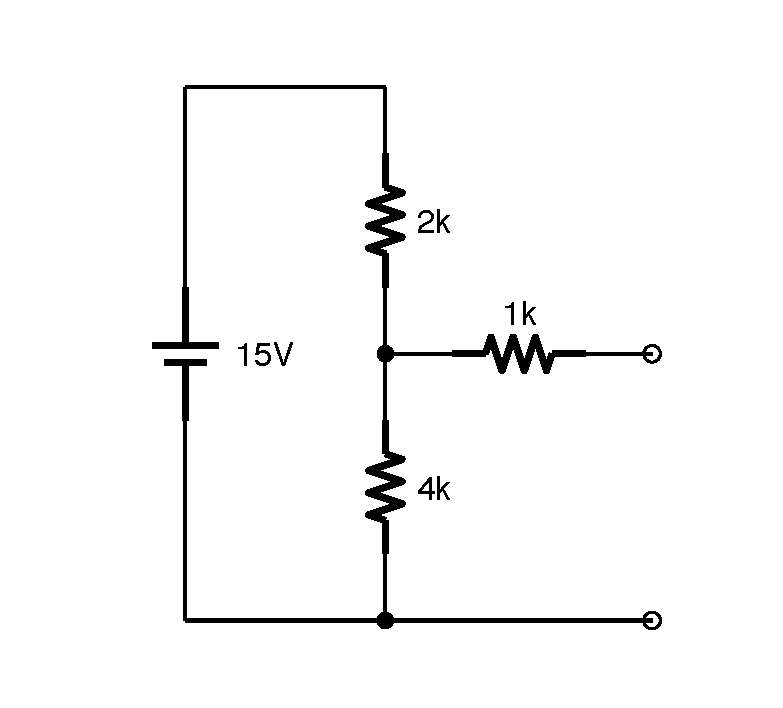
\includegraphics[scale=0.25]{ThevProblem1.pdf}
\item Suppose I have a circuit where, when I add a load of $350\myohm$ I get a $7\myvolt$ drop, and when I add a load of $2000\myohm$ I get an $8\myvolt$ drop.  Calculate and draw the \thev Equivalent circuit.
\end{enumerate}


\end{document}
